%!TEX root = ../thesis.tex
% ******************************* Thesis Appendix A ****************************
\chapter{Formal Definitions} 
\label{appendix:A}

\ifpdf
\graphicspath{{Appendix1/Figs/Raster/}{Appendix1/Figs/PDF/}{Appendix1/Figs/}}
\else
\graphicspath{{Appendix1/Figs/Vector/}{Appendix1/Figs/}}
\fi

\definecolor{Gray}{gray}{0.92}

\newcolumntype{P}[2]{%
	>{\begin{turn}{#1}\begin{minipage}{#2}\small\raggedright\hspace{0pt}}l%
			<{\end{minipage}\end{turn}}%
}
\newcolumntype{R}[2]{%
	>{\columncolor{Gray}}
	>{\begin{turn}{#1}\begin{minipage}{#2}\small\raggedright\hspace{0pt}}l%
			<{\end{minipage}\end{turn}}%
}
\newcolumntype{a}{>{\columncolor{Gray}}c}



\tocless\section{Dynamical systems and notable features}
\label{sec:formal_dyn_sys}

This subsection provides formal definitions for dynamical systems and notable features introduced in Sec.~\ref{subsec:dyn_sys}. Most of definitions and theorems come from and are detailed in \cite{strogatz2018nonlinear, kuznetsov2013elements,Golubitsky2003a,Berglund2006,thompson2011predicting,dobrushkin2014applied}. A dynamical systems is defined as follows:
\begin{definition}
	A \textbf{dynamical system} is a triple $\{\Omega, \phi^t, \mathcal{T}\}$, where $\mathcal{T}$ is a time set, $\Omega$ is a (Banach) state (or \textit{phase}) space with a properly defined metrics on it and $\phi^t: \Omega \to \Omega$ is a family of evolution operators parametrized by $t \in \mathcal{T}$ and satisfying:
	\renewcommand{\theenumi}{\roman{enumi}}%
	\begin{enumerate}
		\item $\phi^0 = id$
		\item $\phi^{t+s} = \phi^t \circ \phi^s$ \text{ ($\circ$ is the convolution operator).}
	\end{enumerate}
\end{definition}
\begin{definition}
	An \textbf{orbit} (or \textbf{trajectory}) starting at $u_0$ is an ordered subset of the state space $\Omega$,
	\begin{equation*}
		\text{Or}(u_0) = \{ u \in \Omega : u = \phi^t u_0, \forall t \in \mathcal{T} \text{ such that } \phi^t u_0 \text{ is defined} \}
	\end{equation*}
\end{definition}
\begin{definition}
	The \textbf{phase portrait} of a dynamical system is a partitioning of the state space into orbits.
\end{definition}
For analysis purposes, one can explicit a dynamical system as a set of differential equations where algebraic operations are well defined. In fact, the main result of the following theorem is that a system of ordinary differential equations can be regarded as a dynamical system\footnote{Another way to represent dynamical systems whose time is discretized are \textit{maps}. However, they are not of primary interest in this thesis.}.
\begin{theorem} \label{th:ODE}
	Consider a system of \textbf{ordinary differential equations}
	\begin{equation}
		\begin{aligned}
			& \dot{u} = f(u,p,t),    &&        u \in \mathbb{R}^n,       &&  p \in \mathbb{R}^m
			\label{eq:ode_general}
		\end{aligned}
	\end{equation}
	where $f: \mathbb{R}^{n} \to \mathbb{R}^{n}$ is smooth in an open region $U \subset \mathbb{R}^{n}$. Then there is a unique function $u = u(t,u_0)$, $u: \mathbb{R} \times \mathbb{R}^{n} \to \mathbb{R}$ that is smooth in $(t,u_0)$ and satisfies, for each $u_o \in U$, the following conditions:
	\renewcommand{\theenumi}{\roman{enumi}}%
	\begin{enumerate}
		\item $u(0,u_0)=u_0$
		\item there is an interval $\mathcal{I}=(-r_1(u_0),r_2(u_0))$, where $r_{1,2}>0$, such that, for all $t \in \mathcal{I}$,
		\begin{equation*}
			y(t) = u(t,u_0) \in U
		\end{equation*}
		and
		\begin{equation*}
			\dot{y} = f(y(t)) '; .
		\end{equation*}
	\end{enumerate}
	The function $u(t,u_0)$ produces a \textbf{solution curve}
	\begin{equation*}
		Cr(u_0) = \{ (t,u):u=u(t,u_0), t\in \mathcal{I} \}  \subset \mathbb{R} \times \mathbb{R}^{n}
	\end{equation*}
	and an orbit 
	\begin{equation*}
		Or(u_0) = \{ u:u=u(t,u_0), t\in \mathcal{I} \}  \subset \mathbb{R}^{n} \, .
	\end{equation*}
	Note that the orbit is the projection of the solution curve onto the state space $\mathbb{R}^{n}$. The evolution operator $\phi^t: \mathbb{R} \to \mathbb{R}$ can thus be written
	\begin{equation*}
		\phi^t u_0 = u(t,u_0)
	\end{equation*}
	As a consequence, we can regard the system of ordinary differential equations like Eq. \ref{eq:ode_general} as a dynamical system. 
\end{theorem}
When \gls{ODE} \ref{eq:ode_general} does explicitly depend on time, it is termed \textit{nonautonomous}; when it does not, it is termed \textit{autonomous}. $u$ are state variables that univocally define the state of the system. $n$ is the system \textit{dimension}, namely the minimum number of state variables (in physics, it is also called the ``number of degrees of freedom''). $m$ represents the number of free parameters that specify the evolution function. The function(s) $f(u,p,t)$ can depend linearly or non-linearly to its variables.




\tocless\section{Slow-fast systems}
\label{sec:slowfast}
Many systems of non-linear \gls{ODE}s are characterized by different time scales. When such time scales are well-defined mathematically, or when we can assume such separation by observing the desired phenomenon, the system can be written as a \textit{slow-fast ODE} in the form:
\begin{align}
	\epsilon \frac{dx}{dt} & = f(x,y)\\
	\frac{dy}{dt} &= g(x,y) \, ,
	\label{eq:slowfast}
\end{align} 
where $0<\epsilon \ll 1$ is a small parameter. $x$ contains fast degrees of freedom and $y$ the slow ones. Alternatively, one can write the system in terms of fast time $s=t/\epsilon$ as
\begin{align}
	\frac{dx_s}{ds} & = f(x_s,y_s)\\
	\frac{dy_s}{ds} &= \epsilon g(x_s,y_s) \, .
\end{align} 
There are different methods to verify the time scale separation in models, the most notable ones involve spectral theory and large deviation theory \citep{Berglund2006}. Empirically, one can consider the rates (or times) in which a process and its coupled ones occur and compare e.g. their orders of magnitude.\\
\begin{definition}
	A \textbf{slow manifold} is a set of equilibria onto which the system is projected if an asymptotically stable equilibrium $\hat{x}(y)$ is admitted for each quasi-steady-state $y$.
	\label{def:slow_man}
\end{definition}
By doing so, the complexity of the system is largely reduced and analytical results can be more easily obtained \citep{strogatz2018nonlinear}. As a matter of fact, as $y$ is almost fixed, one can interpret it a the usual slowly varying parameter $p$. 




\tocless\section{Equilibria, cycles, invariant sets}
\label{sec:equlibria}

\begin{definition}
	A point $\hat{u} \in \Omega$ is called an \textbf{equilibrium point} (fixed point) if $\phi^t\hat{u} = \hat{u}$ for all $t \in \mathcal{T}$.
\end{definition}
Note a slight abuse of wording when referring to ``equilibrium''. In fact, this mathematical term refers to the physical notion of ``steady-state'', given by the no-change condition $\frac{du}{dt} = 0$ in the associated \gls{ODE}. It is different from the mechanical definition of equilibrium as balance of forces acting on the system $\sum_{i} F_i = 0$ or the thermodynamic requirement of absence of net flux of energy though the system $\sum_{i} J_i = 0$ (adiabatic regime).
\begin{definition}
	A \textbf{cycle} is a periodic orbit, that is, a nonequilibrium orbit $Cy$ such that each point $\tilde{u} \in Cy$ satisfies $\phi^{t+\tau}\tilde{u} = \phi^t \tilde{u}$ for all $t \in \mathcal{T}$. The minimal $\tau > 0$ with this property is called the \textit{period} of the cycle.
\end{definition}
\begin{definition}
	A cycle of a continuous-time dynamical system, in a neighbourhood of which there are no other cycles, is called a limit cycle.
\end{definition}
\begin{definition}
	An \textbf{invariant set} of a dynamical system is a subset $\mathcal{S} \subset \Omega$ such that $\tilde{u} \in \mathcal{S}$ implies $\phi^t\tilde{u} \in \mathcal{S}$ for all $t \in \mathcal{T}$.
\end{definition}
An equilibrium point is an invariant set, so is a cycle.
\begin{definition}
	An equilibrium $\hat{u}$ is called \textbf{hyperbolic} (or generic) if there are no eigenvalues of $\partial_u f(u)|_{\hat{u}}$ on the imaginary axis. Otherwise, the equilibrium is called \textbf{elliptic}.
\end{definition}





\tocless\section{Stability}
\label{sec:formal_stability}
We get now into the definition of stability, of primary importance to assess how sensitive a system is to small perturbations.
\begin{theorem}
	An invariant set $\mathcal{S}$ is stable if the following conditions hold:
	\renewcommand{\theenumi}{\roman{enumi}}%
	\begin{enumerate}
		\item for any sufficient small neighbourhood $U \supset \mathcal{S}$ there exist a neighbourhood $V \supset \mathcal{S}$ such that $\phi^tu \in U$ for all $u \in V$ and all $t>0$;
		\item there exist a neighbourhood $U_0 \supset \mathcal{S}$ such that $\phi^tu \to \mathcal{S}$ for all $u \in U_0$, as $t \to +\infty$.
	\end{enumerate}
	\label{theorem:stability}
\end{theorem}
Condition (i) is often called ``Lyapunov stability'', whereas condition (ii) is referred to as ``asymptotic stability''.
A stable invariant set is often called an \textbf{attractor}.
Fixed points and limit cycles are classified as (linearly) stable or unstable depending on the eigenvalues of their associated Jacobian.
\begin{theorem}
	Consider a dynamical system \ref{eq:ode_general}, where $f$ is smooth. Suppose that it has a fixed point $\hat{u}$. Then $\hat{u}$  is (linearly) stable if all eiganvalues $\lambda_1, ..., \lambda_n$ of $\partial_u f(\hat{u})$ satisfy $\operatorname{Re}(\lambda) < 0$.
	\label{theorem:linear_stability}
\end{theorem}

Extracting stability information from determinant, discriminant and trace of the Jacobian is described in Sec.~\ref{subsec:dyn_sys}, along with their graphical representation with a Poincar\'e Diagram, Fig~\ref{fig:poicare}. 






\tocless\section{Bifurcations}
\label{sec:bif_formal}
Mathematically speaking, when the behaviour of a system changes, we encounter a bifurcation. Hence, it is necessary to formalize the notion of ``behaviour'' and that of ``change'' in terms of the elements presented so far. Note that, once the phase space is defined by the state variables, its properties are then given by the parameters introduced in Eq. \ref{eq:ode_general}.
\begin{definition}
	A dynamical system $\{\mathcal{T}, \mathbb{R}^n, \phi^t\}$ is called \textbf{locally topologically equivalent} to a dynamical system $\{\mathcal{T}, \mathbb{R}, \psi^t\}$ if there exist a homeomorphism $h: \mathbb{R}^n \to \mathbb{R}^n$ mapping orbits of the first system to orbits of the second system while preserving the direction of time.
\end{definition}
\begin{definition}
	A dynamical system $\{\mathcal{T}, \mathbb{R}^n, \phi^t\}$ is called \textbf{locally topologically equivalent} near an equilibrium $\hat{u}$ to a dynamical system $\{\mathcal{T}, \mathbb{R}, \psi^t\}$ near an equilibrium $\hat{y}$ if there exist a homeomorphism $h: \mathbb{R}^n \to \mathbb{R}^n$ that:
	\renewcommand{\theenumi}{\roman{enumi}}%
	\begin{enumerate}
		\item is defined in a small neighborhood $U \in \mathbb{R}^n$ of $\hat{u}$;
		\item satisfies $\hat{y} = h(\hat{u})$;
		\item maps orbits of the first system in $U$ onto orbits of the second system in $V=h(U) \subset \mathbb{R}^n$ preserving the direction of time.
	\end{enumerate}	
\end{definition}
\begin{definition}
	The appearance of a topologically non-equivalent phase portrait under variation of parameters is called a \textbf{bifurcation}.
\end{definition}
\begin{definition}
	The \textbf{codimension} of a bifurcation system \ref{eq:ode_general} is the difference between the dimension of the parameter space and the dimension of the corresponding bifurcation boundary.
\end{definition}
\begin{definition}
	A \textbf{bifurcation diagram} of the dynamical system is a stratification of its parameter space induced by the topological equivalence, together with representative phase portraits for each stratum.
	\label{def:bif_diag}
\end{definition}
\begin{definition}
	The \textbf{normal form} of a dynamical system is a simplified form (in scalar system, a function) that can be useful in determining the system's behaviour. All systems exhibiting a certain type of bifurcation are locally (around the equilibrium) topologically equivalent to the normal form of the bifurcation.
\end{definition}
Formally speaking \citep{kuznetsov2013elements}, consider a dynamical system
\begin{equation}
	\dot{x} = f(x,p') \ , \, x\in \mathbb{R}^n \ , \, p' \in \mathbb{R}^n
	\label{eq:dyn_sis}
\end{equation}
and a polynomial system
\begin{equation}
	\dot{\zeta} = g(\zeta,p;\beta) \ , \, \zeta \in \mathbb{R}^n \ , \, p \in \mathbb{R}^k \ , \, \beta \in \mathbb{R}^l
	\label{eq:poly_sys}
\end{equation}
having dimension $n$, codimension $k$ and polynomial order $l$. Without loss of generality, we can assume that the tipping point occurs at $(x,p)=(0,p_0)$. A translation would do it. Then:
\begin{definition}
	System \ref{eq:poly_sys} is called a \textbf{topological normal form} for the bifurcation if any generic system \ref{eq:dyn_sis} with the equilibrium $x=0$ satisfying the same bifurcation conditions at $p' = 0$ is locally topologically equivalent near the origin to \ref{eq:poly_sys} for some values of the coefficients $\beta_i$.
	\label{def:normal_form}
\end{definition}
Here, \textit{generic} means that the system satisfies certain conditions around the critical point: $\frac{\partial^j f}{\partial \varphi^j}|_{(0,p_0)}$, where $j$ is the derivate order and $\varphi = \{x, p\}$. In particular, $\frac{\partial^j f}{\partial x^j}$ are called \textit{nondegeneracy conditions} and are related to the ``criticality'' of a bifurcation \citep{kuehn2011mathematical}, while $\frac{\partial^j f}{\partial p^j}$ are called \textit{trasversality conditions} and govern the bifurcation unfolding (see below) and thus its genericity.

Bifurcations can be divided into two principal classes:
\begin{itemize}
	\item Local bifurcations, which can be analysed through changes in the local stability properties of equilibria, periodic orbits or other invariant sets as parameters cross through critical thresholds;
	\item Global bifurcations, that cannot be detected purely by a stability analysis of the invariant set. They are harder to detect because they involve large regions of the phase plane rather than just the neighbourhood of a single fixed point.
\end{itemize}

One important concept to reduce dynamical systems to local, low-dimensional normal forms is the \textbf{center manifold} \citep{Haragus2010,Crawford1991a}. According to the linearized systems and its stability properties (see above), a dynamical system has invariant manifolds of which one is the center manifold, having the same dimension of the stable manifold (attractor) and tangent to the center subspace at every equilibrium point \citep{Guckenheimer2009a}. A center manifold corresponds to a slow manifold (Def.~\ref{def:slow_man}) when the eigenvalues of the center subspace are all precisely zero, rather than just real part zero. 
\begin{theorem}
	The \textbf{center manifold emergence theorem} says that a neighbourhood around an equilibrium point may be chosen so that all solutions of the system staying in that neighbourhood tend exponentially quickly to some solution $y(t)$ on the center manifold.
	\label{th:centre_man}
\end{theorem}
The theorem allows to reduce complex multi-dimensional dynamics to low dimension dynamics, locally described by bifurcation normal forms. This guarantees that, for stability analysis and related locally ``qualitative'' features, it is sufficient to study bifurcation normal forms and their properties, to which the system reduces and that represent universal (local) routes to phase changes. Generalising centre manifold theorems and techniques to non-autonomous systems \citep{potzsche2006taylor} unleashed, among the others, studies of rate-induced tipping points (Sec.~\ref{sec:classification}).  \\

Models are idealized assumptions of reality (Chapter \ref{ch:intro}). When proved wrong or inadequate, they can be improved by adding small terms that were initially neglected and that would model e.g. impurities or asymmetries in real-world systems.
\begin{definition}
	A model obtained by adding small parameters to a given system is called an \textbf{unfolding} of the original system.
	\label{def:unfolding}
\end{definition}
Unfolding is nicely described in singularity theory \citep{Golubitsky2003a,kuznetsov2013elements}, to which the reader is referred for formal studies involving advanced topological structures whose definition is beyond the scopes of this appendix. Let us now consider those systems with finite codimension with respect to their topological equivalence, and let us limit our attention to the equilibria solutions. Hence, let us focus on bifurcation unfolding.
\begin{definition}
	\label{def:unfoding}
	An \textbf{unfolding} of a dynamical system under static equivalence is one that exhibits all possible bifurcations of the equilibrium (rest) points, up to topological equivalence of the set of equilibria.
\end{definition}
In other terms, it investigates what happens when small terms are added to the original bifurcation, mimicking extra parameters, small offsets or ``impurities''.
\begin{definition}
	A (local) bifurcation is said to be \textbf{generic} if it results from the unfolding of other bifurcations and does not result in other bifurcations if unfolded.
	\label{def:generic_bif}
\end{definition}





\tocless\section{Critical normal forms}
\label{sec:normal_form}


As anticipated in Def.~\ref{def:normal_form}, a normal form characterises a topological equivalence to bifurcations observed in complex systems. Hence, it locally retains the qualitative features (stability, sensitivity to small perturbations, etc.), in a more compact and analytically tractable form. In addition, according to the centre manifold theorem \ref{th:centre_man}, bifurcation normal forms are adequate descriptors of multi-dimensional dynamical systems near equilibrium points. In this regard, they have often been called ``universal patterns'' to critical and explosive phenomena \citep{Thom2554,Kuehn2021}.

Reducing a system to its (local) normal form may involve different techniques. direct and general center manifold calculation \citep{Guckenheimer2009a,Kuehn2021}. A simpler technique is Taylor expansion around $x \sim x_c$ and $p \sim p_c$ up to second or third order \citep{strogatz2018nonlinear}: 
\begin{equation}
	\dot{x} = f(x,p) = f(x_c, p_c) +(x-x_c) \left. \frac{\partial f}{\partial x} \right\rvert _{(x_c,p_c)} + (p-p_c)\left. \frac{\partial f}{\partial p} \right\rvert _{(x_c,p_c)} + \frac{1}{2} (x-x_c)^2 \left. \frac{\partial^2 f}{\partial x^2} \right\rvert _{(x_c,p_c)} + \dots \, , \label{eq:nf_derivation}
\end{equation}
where subscript $c$ identifies ``critical'' values. However, this procedure is not always possible and it is often necessary to hypothesise the bifurcation to decide which order to truncate in the expansion. Graphical inspection might help crafting the hypothesis by checking how the diagram $(f(x,p),x)$ changes while varying $p$ and comparing its local properties next to the x-axis with those of normal forms (reported below). An example is provided in Fig.~\ref{fig:local_quadratic}. It analyses a harvested population model from \textcite{Scheffer2009}:
\begin{equation}
	\frac{dX}{dt} = X\left(1-\frac{X}{K}\right) - c' \frac{X^2}{X^2+1} \, ,
	\label{eq:harv_pop1}
\end{equation}
where $X$ is population density, $K$ is the carrying capacity and $c'$ is the maximum harvest rate.

Another common option is the spectral analysis of the Jacobian (Sec.~\ref{sec:formal_stability}) and the verification of specific conditions ( listed below) defining each normal form \citep{strogatz2018nonlinear}. A web service curated by prof. A. J. Roberts (\url{http://www.maths.adelaide.edu.au/anthony.roberts/sdenf.php})  provides assistance by solving the computer algebra for a range of finite-dimensional systems. \\


\begin{figure}[h]
	\centering
	\begin{minipage}[c]{0.32\textwidth}
		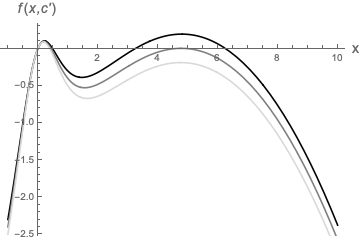
\includegraphics[width=0.9\linewidth]{harv_pop}
		\renewcommand{\figurename}{Fig.}
	\end{minipage}
	\begin{minipage}[c]{0.32\textwidth}
		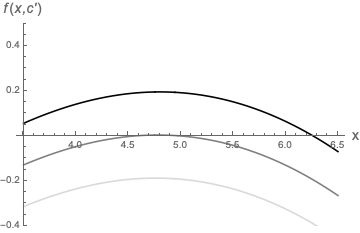
\includegraphics[width=0.9\linewidth]{harv_pop2}
		\renewcommand{\figurename}{Fig.}
	\end{minipage}
	\hspace{0.05cm}
	\begin{minipage}[c]{0.32\textwidth}
		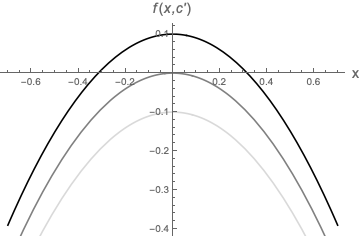
\includegraphics[width=0.9\linewidth]{fold_gray}
		\renewcommand{\figurename}{Fig.}
	\end{minipage} 
	
	\caption{\small \textbf{Left}: graph representation of $f(x,c')$, at different values of $c'$, for model \ref{eq:harv_pop1}. \textbf{Centre:} zoom-in the the previous plot, around $x \simeq 0.47$, to compare with the next plot. \textbf{Right:} sketch of fold vector field (\textit{cf.} Fig.\ref{fig:fold_diag}, right) for different values of $c'$. Compare it with the centre plot: when $c'$ is varied, both graphs move from black to light gray. Although $(X_0,c_0) \neq (0,0)$ due to translations and specific quantitative properties of the realistic model, the qualitative behaviour around the bifurcation is the same.}
	\label{fig:local_quadratic}
\end{figure}



The remaining of this section lists and briefly discusses the normal forms (Def.~\ref{def:normal_form}) of the main low-dimensional bifurcations. Each normal form is presented as $\dot{x} = f(x,p)$ and accompanied by figures about $ f(x,p)$ and its bifurcation diagram\footnote{Plots for bifurcation diagrams and vector fields are adapted from Suba Thomas, "Bifurcation Diagrams with Flow Fields" \url{http://demonstrations.wolfram.com/BifurcationDiagramsWithFlowFields/}, Wolfram Demonstrations Project, Published: March 7 2011.} $(\tilde{x}, p)$. We also list the critical sowing down (\gls{CSD}) scaling of each bifurcation,  anticipated in Sec.~\ref{sec:mathematical_background} and further discussed in Sec~.\ref{sec:o-u}. In addition to critical bifurcations, the supercritical pitchfork bifurcation has been added for its importance as a counterexample, for its historical connection to second-order phase transitions and for its potential relevance in the biological disciplines, \textit{cf.} Sec.~\ref{sec:beyond_waddington}. Further reading in \textcite{kuznetsov2013elements,strogatz2018nonlinear}. \\


\tocless\subsection{Fold (saddle-node)}
\label{subsec:fold}
This is the basic mechanism by which fixed points are created and destroyed. A fold (or saddle-node, or ``blue-sky'') bifurcation is characterized by the following conditions for a dynamical system $f(x,p)$:

\begin{table}[h!]
	\centering
	\begin{tabular}{ll}
		$\frac{\partial f}{\partial x}(0,p_0)  = 0$ & $\frac{\partial f}{\partial p}(0,p_0) \neq 0$   \\
		$\frac{\partial^2 f}{\partial x^2}(0,p_0)  \neq 0$ &   
	\end{tabular}
\end{table}

%\begin{align}
%	\nonumber \frac{\partial f}{\partial x}(0,p_0) & = 0\\
%	\nonumber \frac{\partial^2 f}{\partial x^2}(0,p_0) & \neq 0\\
%	\nonumber \frac{\partial f}{\partial p}(0,p_0) & \neq 0
%\end{align} 
\noindent The fold is a 1-dimension, 1-codimension bifurcation. Its normal form is:
\begin{equation}
	\dot{x} = p+x^2 \, .
	\label{eq:fold}
\end{equation}
For $p<0$, there are two equilibria $\hat{x}_{1,2} = \pm \sqrt{-p}$. $\hat{x}_1$ is stable and $\hat{x}_2$ is unstable. For $p>0$ there are no equilibria in the system. When $p=0$ the two equilibria collide and disappear, so $p_0 =0$ is the critical value for the parameter.
\begin{remark}
	The system $\dot{x} = p-x^2$ can be considered the same way, as well as any system mapped with $x \rightarrow -x$ and $p \rightarrow -p$.
	\label{rem:fold}
\end{remark}
\begin{lemma}
	Near the origin, the system $\dot{x} = p+x^2 + O(x^3)$ is locally topologically equivalent to the system $\dot{x} = p+x^2 $.
	\label{lemma:fold}
\end{lemma}

To visualize how $f(x,p)$ is varied under the action of $p$, see Fig. \ref{fig:fold_diag} (left). The fold mechanism is given by a translation, driven by $p$, of $f(x,p)$ across the 0-axis, that destroys (or creates, depending on the direction) the equilibria. In addition, Fig. \ref{fig:fold_diag} (centre) shows the evolution of the associated analytical potential $V(x,p) \, \text{s.t.} \, f(x,p) = - \frac{\partial V}{\partial x}$ while $p$ is varied. It it straightforward to associate it to the ``pebble-down-the-hill'' analogy (see Sec. \ref{subsec:pebble}).  Fig. \ref{fig:fold_diag} (right) shows the fold normal form bifurcation diagram, that displays the picture at once. For each value of the parameter there are different equilibria. Solid lines: stable equilibria; dashed lines: unstable equilibria. $(x,p)=(0,0)$ is the critical point.

\textsc{CSD Scaling}:
\begin{equation}
	u' = \partial_x(p+x^2)|_{\hat{x} = \sqrt{-p}}u = -2\sqrt{-p}u = \mathcal{O}(p^{1/2}) u \, .
\end{equation}
Therefore the recovery exponent is $\alpha = 1/2$, that is, perturbations get recovered with rate proportional to the square root of the parameter. If $p \rightarrow 0$, the speed of recovery goes to zero as well, hence the ``Slowing Down'' phenomenon.

\begin{figure}[h]
	\centering
	\begin{minipage}[c]{0.32\textwidth}
		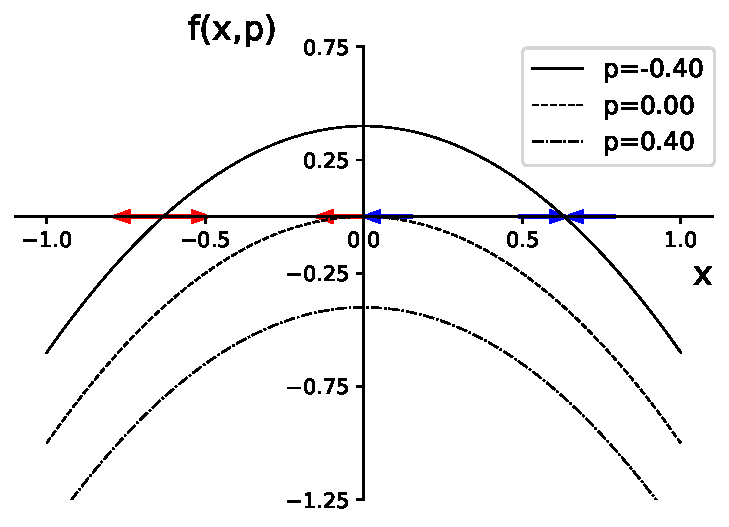
\includegraphics[width=\linewidth]{fold_v}
		\renewcommand{\figurename}{Fig.}
	\end{minipage}
	\hspace{0.01cm}
	\begin{minipage}[c]{0.32\textwidth}
		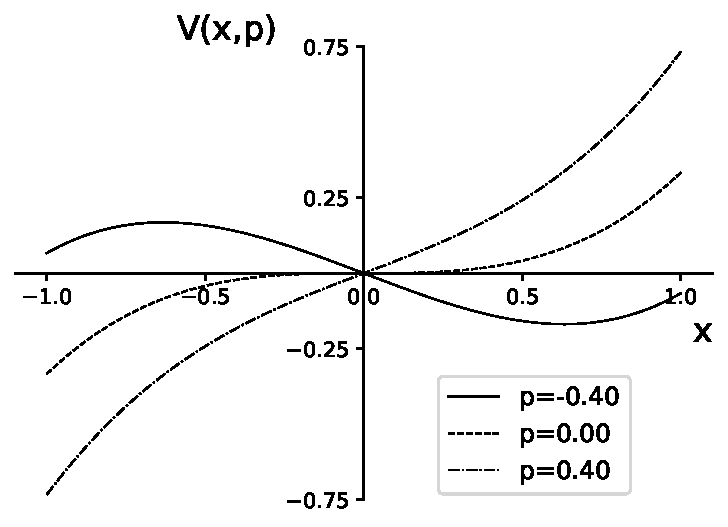
\includegraphics[width=\linewidth]{fold_p}
		\renewcommand{\figurename}{Fig.}
	\end{minipage} 
	\hspace{0.01cm}
	\begin{minipage}[c]{0.32\textwidth}
		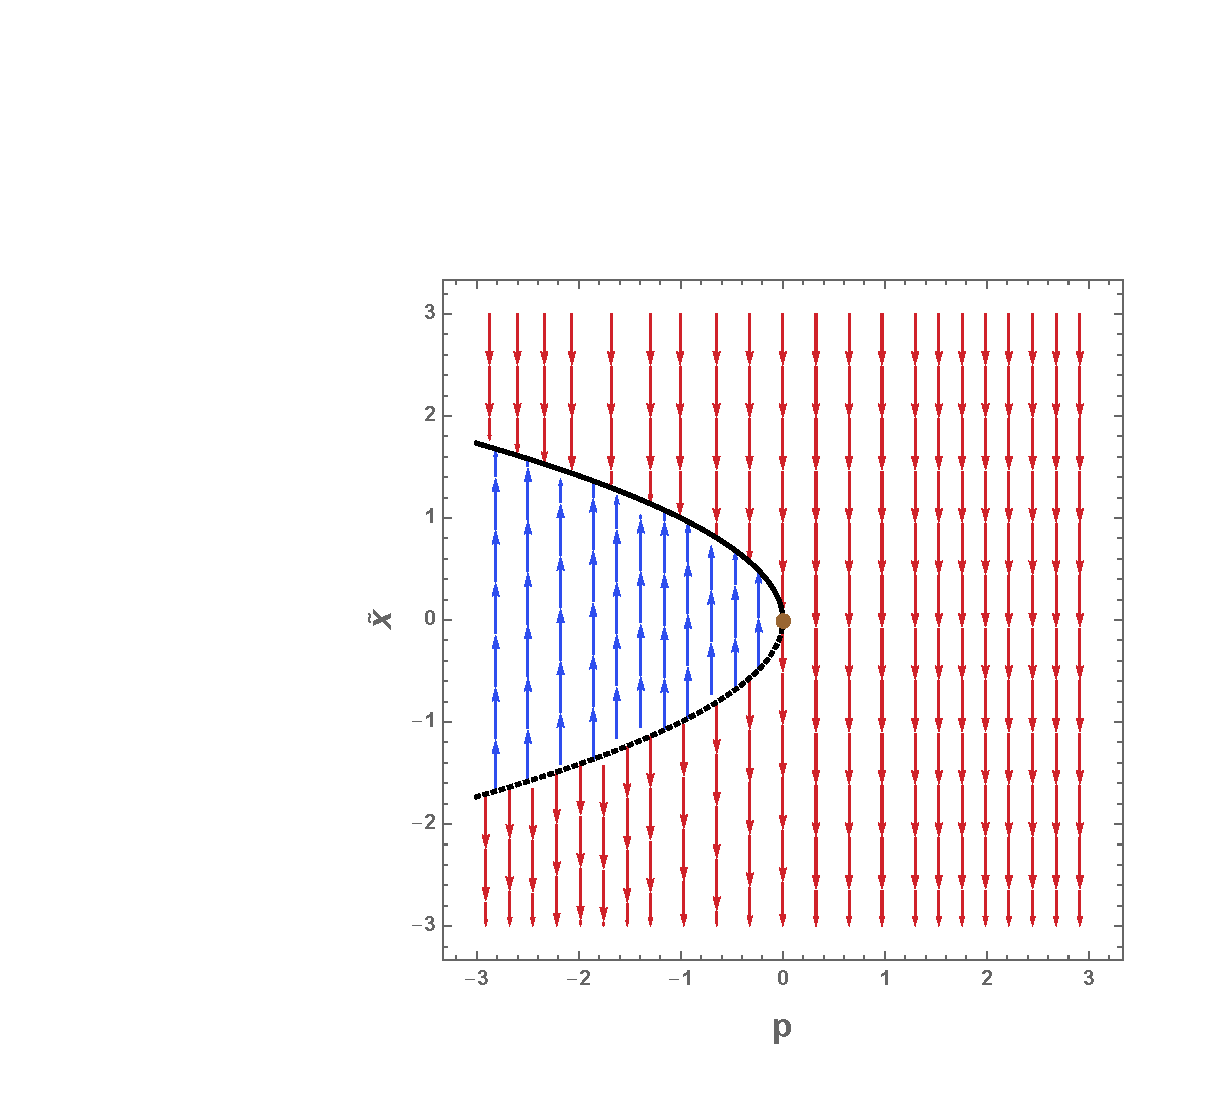
\includegraphics[width=0.85\linewidth]{fold_bd}
		\renewcommand{\figurename}{Fig.}
	\end{minipage}
	
	\caption{\small \textbf{Left:} evolution of $f(x,p)$ for a fold normal form, when $p$ changes from negative to positive values. Red diverging arrows indicate the direction of instability; blue converging arrows that of stability. For $p = p_0 = 0$ a saddle node is created, with a stable and an unstable direction. \textbf{Centre:} quasi-steady state potential $V(x,p)$ for different values of $p$. For $p<0$, a stable steady-state is present (valley); that becomes flat when $p=0$ and unstable for $p>0$. In the latter case, the ``pebble'' will roll down towards another, far away equilibrium. \textbf{Right:} bifurcation diagram of the fold normal form \ref{eq:fold}. The equilibrium manifold is in black (solid line: stable; dashed: unstable).Vector field lines indicate whether the system is pushed upwards or downwards. }
	\label{fig:fold_diag}
\end{figure}


\tocless\subsection{Transcritical}
There are certain situations when a fixed point always exist (e.g. populations with zero individuals will never grow even thought the growth rate increases); however, such equilibrium changes stability. Transcritical bifurcations does the job by following the conditions:

\begin{table}[h!]
	\centering
	\begin{tabular}{ll}
		$\frac{\partial f}{\partial x}(0,p_0)  = 0$ & $\frac{\partial^2 f}{\partial x \partial p}(0,p_0)  \neq 0$   \\
		$\frac{\partial^2 f}{\partial x^2}(0,p_0) \neq 0$ &   $\frac{\partial f}{\partial p}(0,p_0) = 0$
	\end{tabular}
\end{table}

%\begin{align}
%	\nonumber \frac{\partial f}{\partial x}(0,p_0) & = 0\\
%	\nonumber \frac{\partial^2 f}{\partial x^2}(0,p_0) & \neq 0\\
%	\nonumber \frac{\partial^2 f}{\partial x \partial p}(0,p_0) & \neq 0\\
%	\nonumber \frac{\partial f}{\partial p}(0,p_0) & = 0
%\end{align} 
The associated normal form is:
\begin{equation}
	\dot{x} = px-x^2 \, .
	\label{eq:transcritical}
\end{equation}
It has one fixed equilibrium at $\hat{x}_1 = 0$ that switches stability according to the sign of $p$, while the other equilibrium is $\hat{x}_2 =p$ and changes stability in reverse order as compared to $\hat{x}_1$. The evolution of $f(x,p)$ with respect to the parameter looks as in Fig. \ref{fig:trans_diagram}. The bifurcation diagram is depicted in Fig. \ref{fig:trans_diagram_bif}. 

\textsc{CSD Scaling:}
\begin{equation}
	u' = \partial_x(px-x^2)|_{\hat{x} = 0}u = \mathcal{O}(p) u \ , \ \alpha =1 \, .
\end{equation}



\begin{figure}[h!]
	\centering
	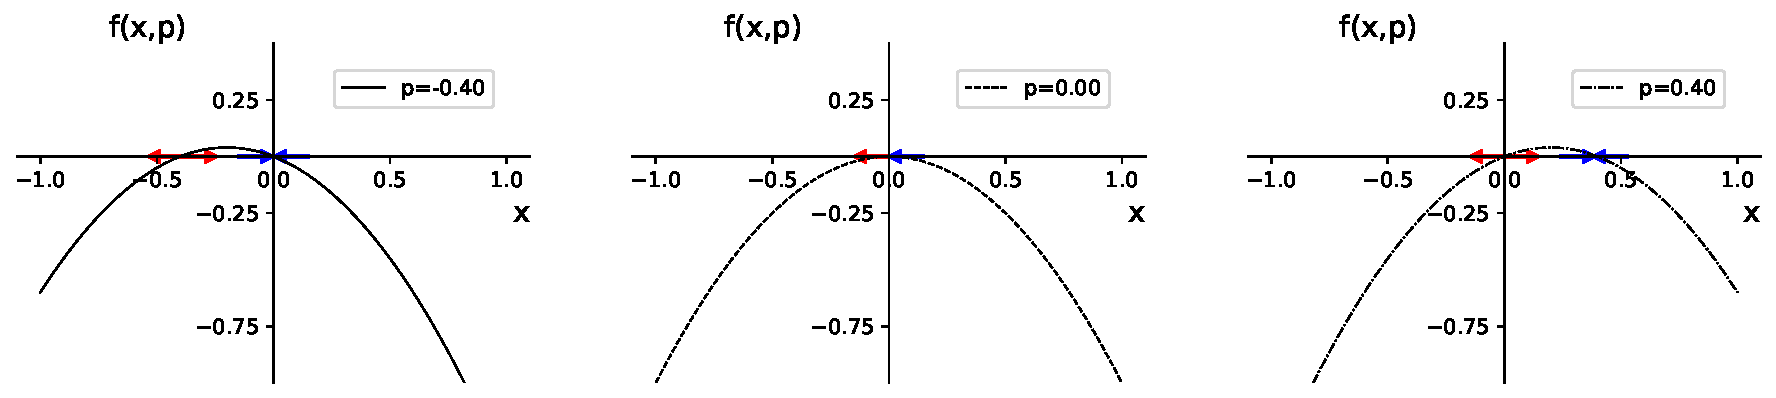
\includegraphics[width=\linewidth]{trans_v}
	\caption{\small Evolution of $f(x,p)$ for a transcritical normal form when $p$ changes from negative to positive values. $f(x,p)$ moves in a tilting fashion. Red diverging arrows indicate the direction of instability; blue converging arrows that of stability. $p=0$ is the critical value. }
	\label{fig:trans_diagram}
\end{figure}


\begin{figure}[h!]
	\centering
	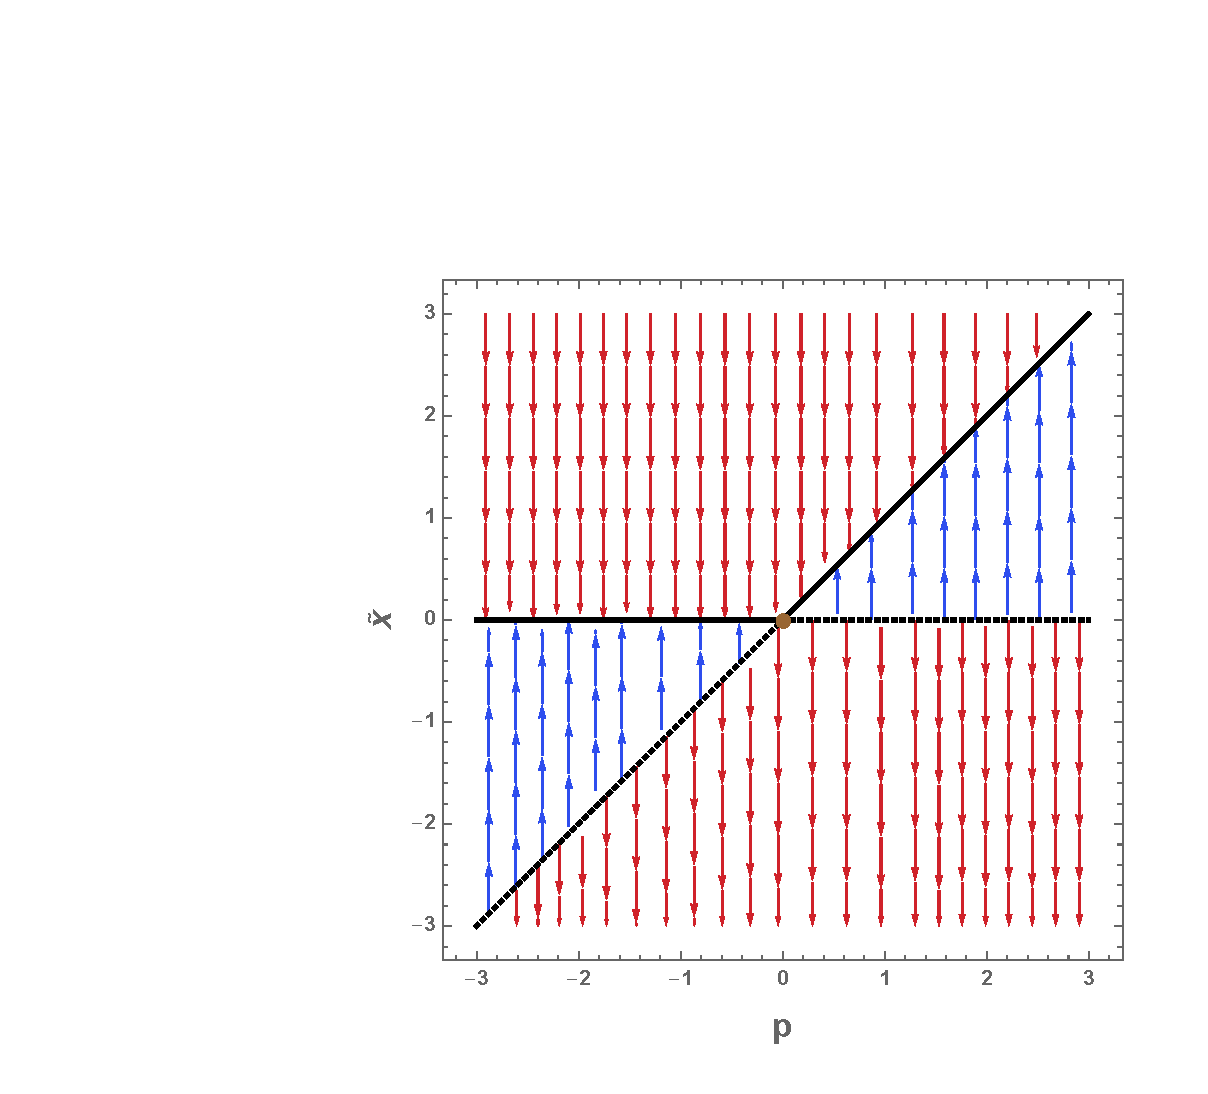
\includegraphics[width=0.34\linewidth]{trans_bd}
	\caption{\small Bifurcation diagram of the transcritical normal form \ref{eq:transcritical}. The equilibrium manifold is in black (solid line: stable; dashed: unstable).Vector field lines indicate whether the system is pushed upwards or downwards. }
	\label{fig:trans_diagram_bif}
\end{figure}







\tocless\subsection{Subcritical pitchfork}
This is common in problems where there is symmetry (e.g. spatial symmetry) so that the system can choose in which equilibrium to converge. Generic conditions are:

\begin{table}[h!]
	\centering
	\begin{tabular}{ll}
		$ -f(x,p) = f(-x,p) \, \text{(symmetry)}$ & $\frac{\partial^2 f}{\partial x \partial p}(0,p_0)  \neq 0$   \\
		$\frac{\partial f}{\partial x}(0,p_0) = \frac{\partial^2 f}{\partial x^2}(0,p_0) =  \frac{\partial f}{\partial p}(0,p_0) = 0$ &   $\frac{\partial^3 f}{\partial x^3 }(0,p_0)  > 0$
	\end{tabular}
\end{table}
%\begin{align}
%	\nonumber & -f(x,p) = f(-x,p) \, (symmetry)\\
%	\nonumber & \frac{\partial f}{\partial x}(0,p_0) = \frac{\partial^2 f}{\partial x^2}(0,p_0) =  \frac{\partial f}{\partial p}(0,p_0) = 0\\
%	\nonumber & \frac{\partial^2 f}{\partial x \partial p}(0,p_0)  \neq 0\\
%	\nonumber & \frac{\partial^3 f}{\partial x^3 }(0,p_0)  > 0\\
%\end{align} 

Its normal form is:
\begin{equation}
	\dot{x} = px + x^3 \, .
	\label{eq:subpitch}
\end{equation}
It has three equilibria for $p<0$, of which $\tilde{x}_3 =0$ is stable and two symmetrical $\tilde{x}_{1,2} = \pm \sqrt{-p}$ are unstable. After $p_0$, the unstable points collide with the stable one and vanish, while $\tilde{x}_3$ becomes unstable. Thus, trajectories diverge to infinity. The evolution of $f(x,p)$ is depicted in Fig. \ref{fig:subpitch_diagram}. Fig.~\ref{fig:subpitch_diagram_bif} shows its bifurcation diagram.

\textsc{CSD Scaling}
\begin{equation}
	u' = \partial_x(px+x^3)|_{\hat{x} = 0}u = \mathcal{O}(p) u \ , \ \alpha =1 \, .
\end{equation}


\begin{figure}[h!]
	\centering
	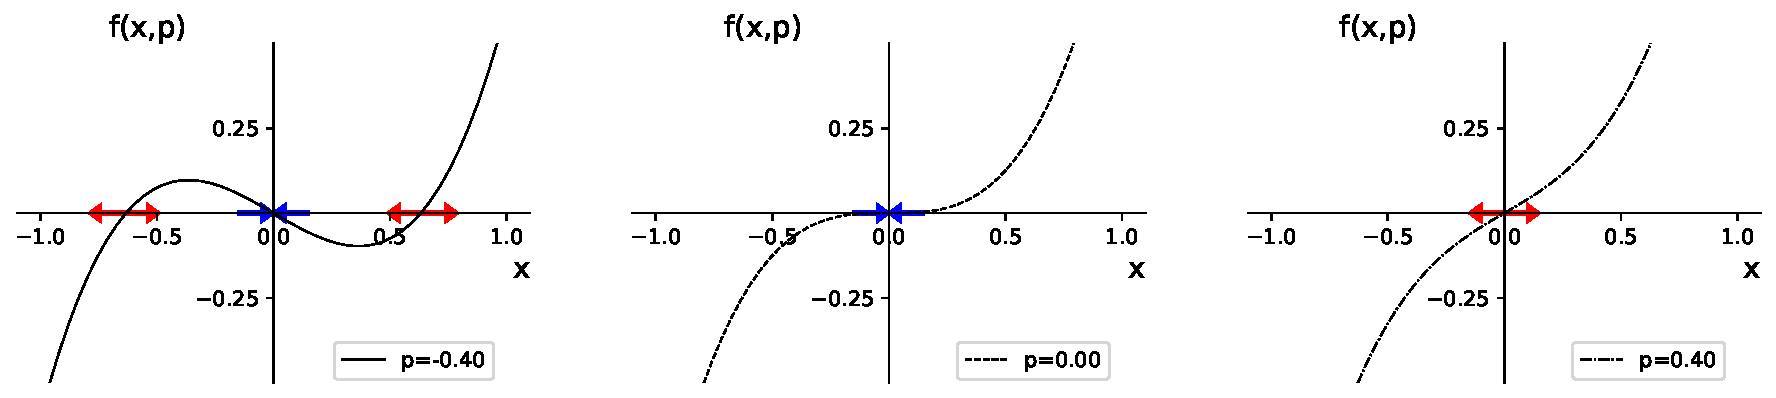
\includegraphics[width=\linewidth]{subpitch_v}
	\caption{\small Evolution of $f(x,p)$ for a subcritical pitchfork normal form when $p$ changes from negative to positive values. Red diverging arrows indicate the direction of instability; blue converging arrows that of stability. $p=0$ is the critical value. }
	\label{fig:subpitch_diagram}
\end{figure}

\begin{figure}[h!]
	\centering
	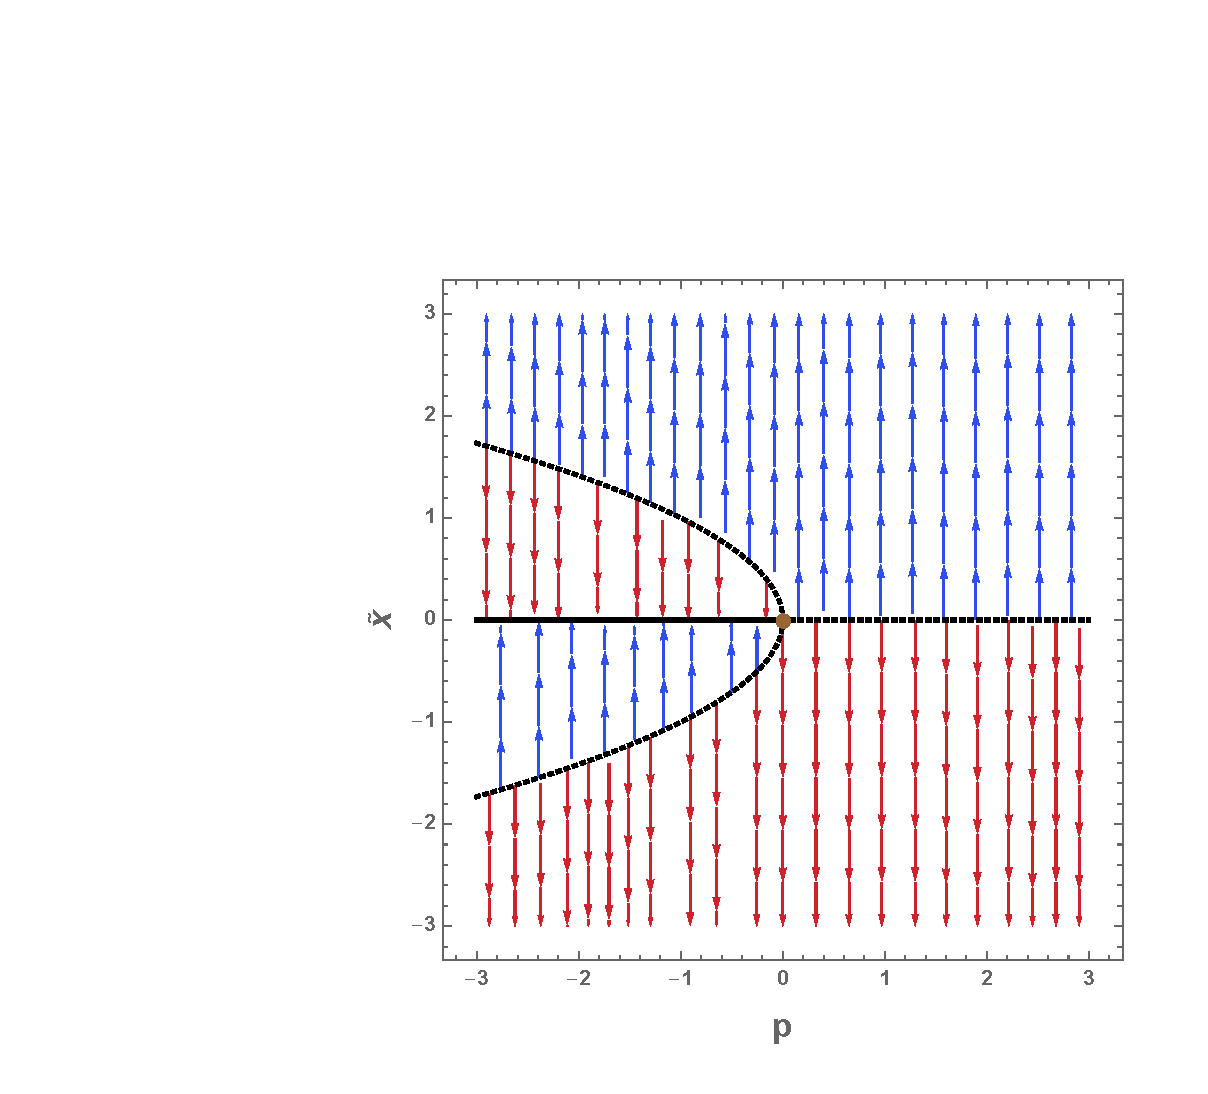
\includegraphics[width=0.34\linewidth]{subpitch_bd}
	\caption{\small Bifurcation diagram of the subcritical pitchfork normal form \ref{eq:subpitch}. The equilibrium manifold is in black (solid line: stable; dashed: unstable).Vector field lines indicate whether the system is pushed upwards or downwards. }
	\label{fig:subpitch_diagram_bif}
\end{figure}



When zooming out the purely local behaviour of real systems, the explosive instability is often counterbalanced by the stabilizing influence of higher order terms. To respect the symmetry conditions, $\mathcal{O}(x^5)$ is then inserted in Eq. \ref{eq:subpitch} to obtain the canonical form of a global subcritical pitchfork:
\begin{equation}
	\dot{x} = px +x^3 -x^5 \, .
	\label{eq:subpitch_global}
\end{equation}
Coefficients of higher order terms can be considered $=1$ after proper non-dimensionalization. Fig.~\ref{fig:subpitch_global} (left) displays $f(x,p)$ for different values of $p$ and unravels local mechanisms analogue to systems \ref{eq:subpitch} (close to $x=0$) and \ref{eq:fold} (close to $x \sim \pm 0.8$). The bifurcation diagram of system \ref{eq:subpitch_global} is shown in Fig. \ref{fig:subpitch_global} (right) after numerical estimation. A subcritical pitchfork bifurcation is a key mechanism to produce tri-stability (co-existence of three stable points) and sharp transitions between attractors. Fig. \ref{fig:subpitch_global} (right) shows hysteresis as effect of non-reversibility of the process. Imagine starting at $(p,\tilde{x})=(-1,0)$ and increasing the parameter. When $p=p_0=0$ the system jumps on the upper or lower branch, mostly depending on random fluctuations. Then, to go back to its original state, it is necessary to decrease the parameter values \textit{below} $p=0$, finally getting to a fold point and having a second abrupt shift towards the origin. The evolution of its associated potential is reported in Fig. \ref{fig:subpitch_global} (centre). We can observe a vanishing tri-stability when $p=0$, which then settles into bistability. That, however, it reached in a critical manner, not smoothly as for a supercritical pitchfork bifurcation (see below).


\begin{figure}[h]
	\centering
	\begin{minipage}[c]{0.32\textwidth}
		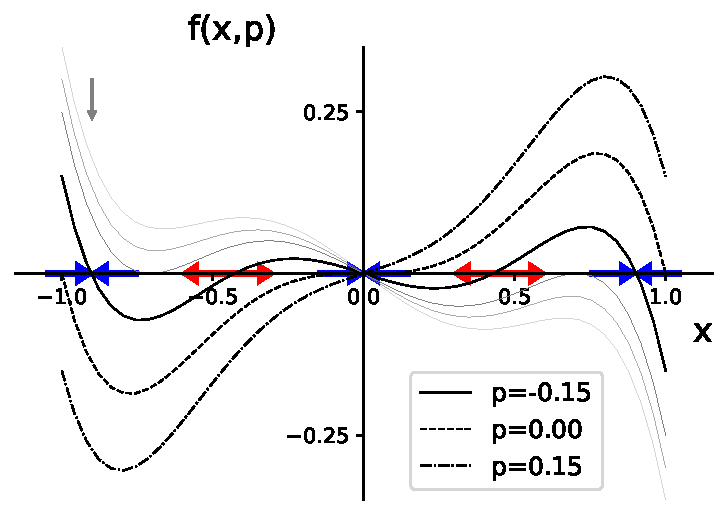
\includegraphics[width=\linewidth]{subpitch_global_v}
		\renewcommand{\figurename}{Fig.}
	\end{minipage}
	\hspace{0.01cm}
	\begin{minipage}[c]{0.32\textwidth}
		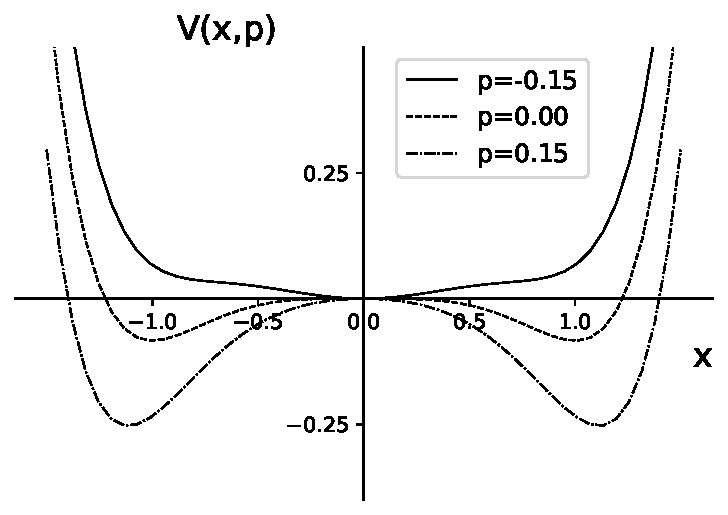
\includegraphics[width=\linewidth]{subpitch_global_p}
		\renewcommand{\figurename}{Fig.}
	\end{minipage} 
	\hspace{0.01cm}
	\begin{minipage}[c]{0.32\textwidth}
		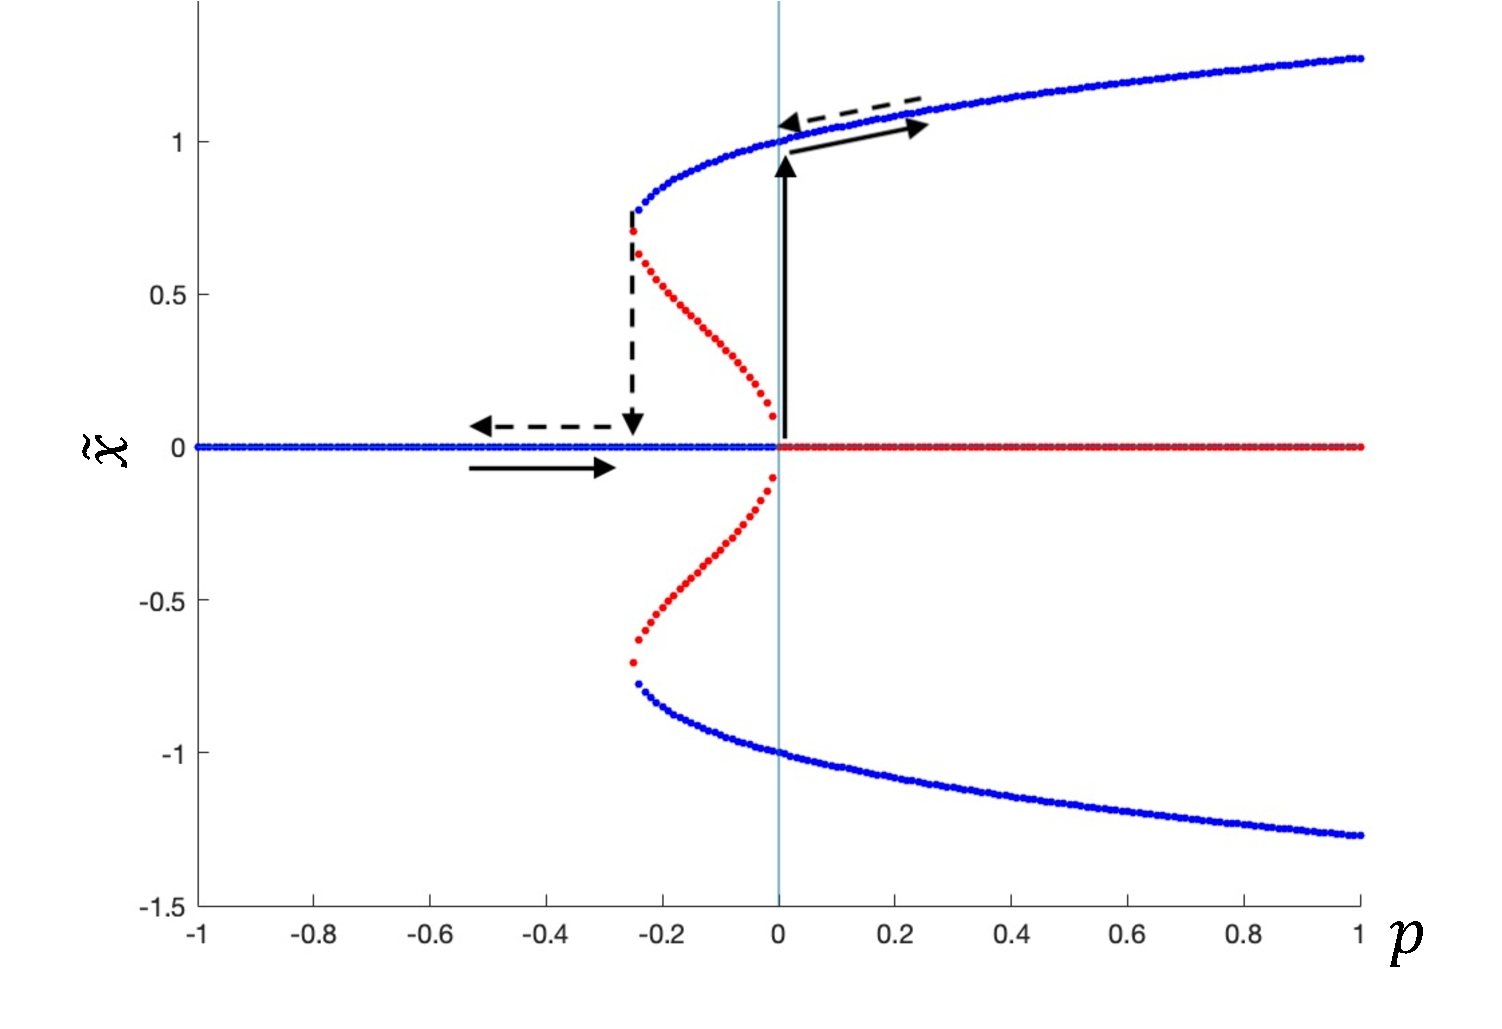
\includegraphics[width=\linewidth]{sub-pitchfork.pdf}
		\renewcommand{\figurename}{Fig.}
	\end{minipage}
	
	\caption{\small \textbf{Left:} evolution of $f(x,p)$ for a global subcritical pitchfork form, when $p$ changes from negative to positive values. Red diverging arrows indicate the direction of instability; blue converging arrows that of stability, in the case of $p=-0.15$. Close to $x=0$, the behaviour is the same as in Fig. \ref{fig:subpitch_diagram_bif}. Further from it, the local behaviour is topologically equivalent to that of a saddle-node. To observe that, follow the light grey plots along the direction pointed by the arrow. Close to $x=-0.8$ and $x=0.8$, the ``hunchbacks'' approach the x-axis with a similar mechanism to that in Fig.~\ref{fig:fold_diag}. They correspond to the local fold bifurcations marked in the bifurcation diagram. \textbf{Centre:} quasi-steady state potential $V(x,p)$ for different values of $p$. For $p<0$, a stable steady-state is present (valley); that becomes flat when $p=0$ (while other two stable states exist) and unstable for $p>0$, where only the two extreme stable states reman. \textbf{Right:} bifurcation diagram of the global subcritical pitchfork normal form \ref{eq:subpitch_global}, estimated with custom numerical methods. Red branches: unstable; blue: stable. Solid arrows indicate the directions followed when $p$ is increased. Dashed lines: directions followed when $p$ is decreased.}
	\label{fig:subpitch_global}
\end{figure}





\tocless\subsection{Supercritical pitchfork}
\label{app:supercr}
Although not strictly critical in the sense of \gls{CT}s \citep{Kuehn2011}, the supercritical pitchfrok bifurcation is worth being studied for several reasons. First, it provides an example of smooth transition in the first derivate of the potential (whereas critical transitions are discrete); hence, it allows to directly compare its notable features with those of ``more'' critical bifurcations. This helps in distinguishing necessary and sufficient conditions for the application of \gls{EWS} \citep{Kefi2013a,Dutta2018}. Second, it is historically relevant as it connects to second-order phase transitions studied in statistical mechanics and thus provides mutual insights \citep{pathria}. The conditions determining a supercritical pitchfork bifurcation are:
\begin{table}[h!]
	\centering
	\begin{tabular}{ll}
		$ -f(x,p)  = f(-x,p)\, \text{(symmetry)}$ & $\frac{\partial^2 f}{\partial x^2}(0,p_0) = 0$   \\
		$\frac{\partial f}{\partial x}(0,p_0) = 0$ &   $\frac{\partial f}{\partial p}(0,p_0) = 0$ \\
		$\frac{\partial^2 f}{\partial x \partial p}(0,p_0)  \neq 0$ &  $\frac{\partial^3 f}{\partial x^3 }(0,p_0)  < 0$
	\end{tabular}
\end{table}

The last condition distinguishes the supercritical from the subcritical case, in a way that makes the former case stable and the latter unstable and thus critical \citep{kuehn2011mathematical}. Following the conditions, its normal form is:
\begin{equation}
	\dot{x} = px-x^3 \, .
	\label{eq:suppitch}
\end{equation}
It is characterized by one stable point $\tilde{x}_3 = 0$ for $p<0$ that becomes unstable at $p_0$, while two other stable points $\tilde{x}_{1,2}$ appear. It is the main mechanism that continuously creates bistability, in a way that one single attractor splits in two as the control parameter is varied, thus allowing different configurations for the system. However, this transition is not abrupt and no hysteresis is present. As mentioned, the mechanism is associated with second-order phase transitions in Statistical Mechanics \cite{strogatz2018nonlinear}.  \\
Fig. \ref{fig:superpitch_diagram} shows the evolution of $f(x,p)$ and Fig. \ref{fig:superpitch_diagram_bif} (left) its associated bifurcation diagram. In addition, Fig. \ref{fig:superpitch_diagram_bif} (right) reports the evolution of the associated potential. \\
It is interesting to compare it with that of the subcritical pitchfork bifurcation (Fig. \ref{fig:superpitch_diagram_bif}, right), in that both potentials evolve towards a two-state equilibrium, but the mechanism (around the bifurcation values) is strikingly different when considering the smoothness of the transition, its reversibility and the co-existance of multiple states. These characteristics are also reflected when small perturbations are considered (see section below) and inform the modelling of processes with similar asymptotic states but different evolution mechanisms.

\textsc{CSD Scaling}
\begin{equation}
	u' = \partial_x(px-x^3)|_{\hat{x} = 0}u = \mathcal{O}(p) u \ , \ \alpha =1 \, .
\end{equation}
Which is indicative for the fact that also non-critical (CT-wise) transitions have CSD and thus can exhibit Early Warning Signals, as discussed in Sec.~\ref{subsec:ews_non_critical}.


\begin{figure}[h!]
	\centering
	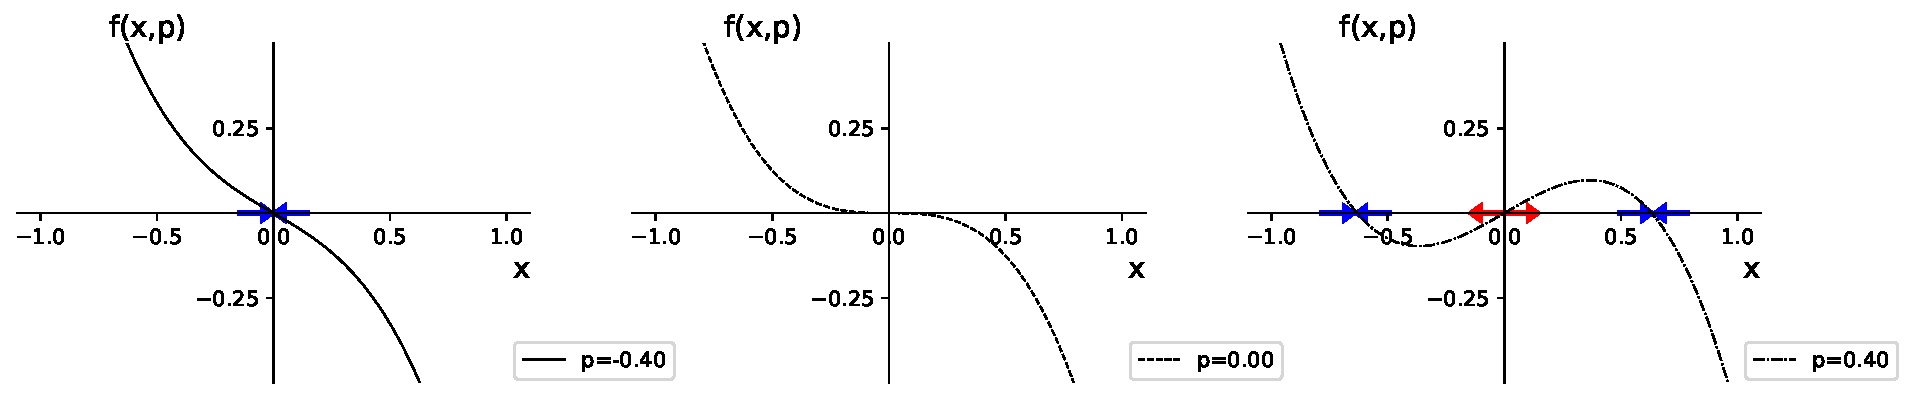
\includegraphics[width=\linewidth]{superpitch_v}
	\caption{\small Evolution of $f(x,p)$ for a supercritical pitchfork normal form when $p$ changes from negative to positive values. Red diverging arrows indicate the direction of instability; blue converging arrows that of stability. $p=0$ is the critical value. }
	\label{fig:superpitch_diagram}
\end{figure}


\begin{figure}[h!]
	\centering
	\begin{minipage}[c]{0.49\textwidth}
		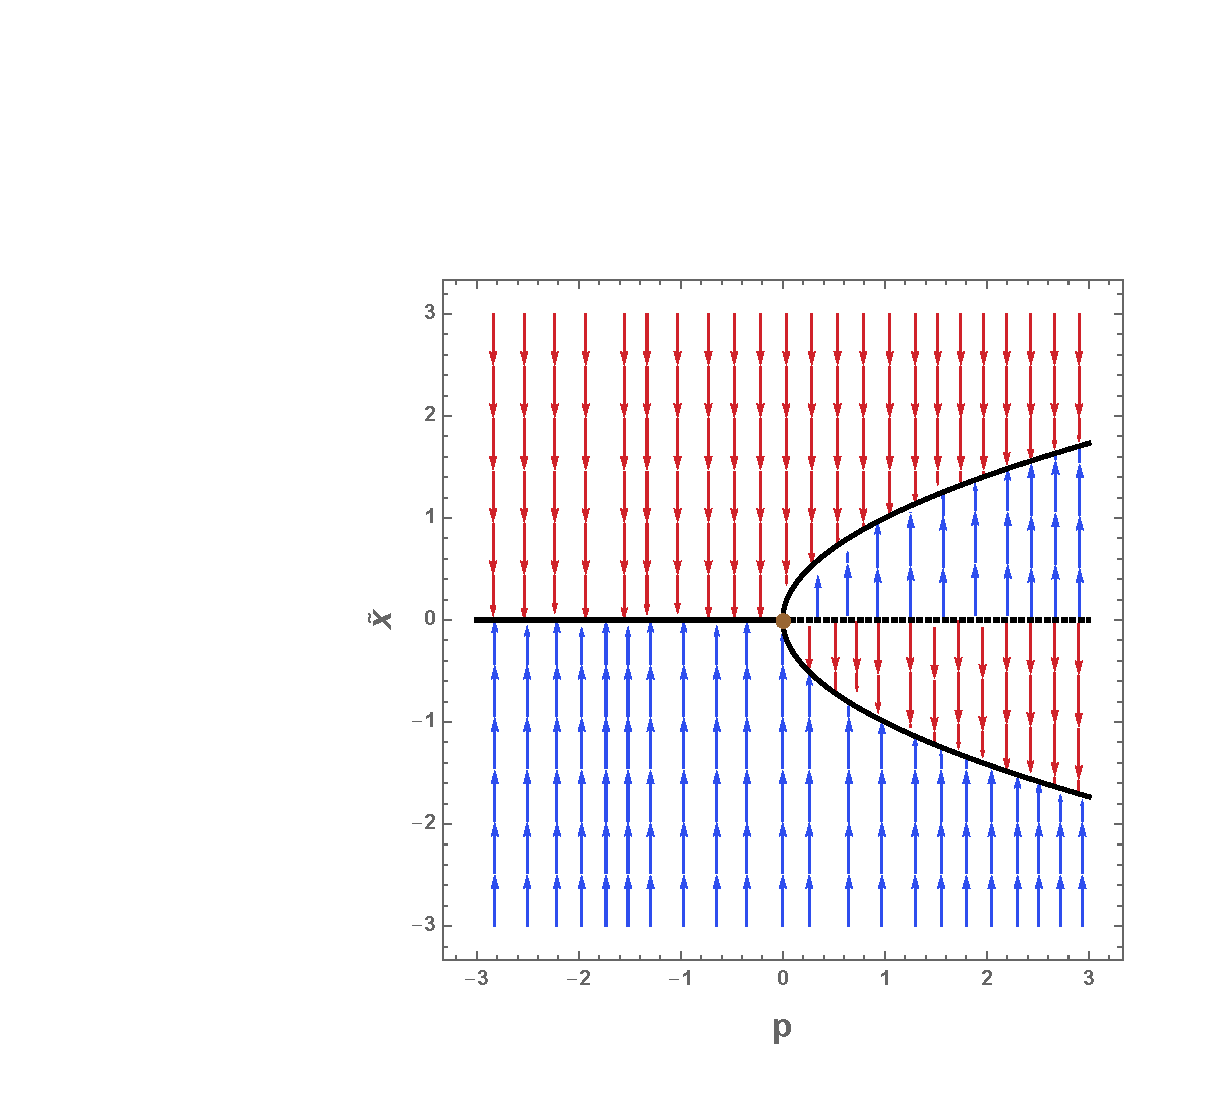
\includegraphics[scale=0.35]{superpitch_bd}
		\renewcommand{\figurename}{Fig.}
	\end{minipage}
	\hspace{0.05cm}
	\begin{minipage}[c]{0.49\textwidth}
		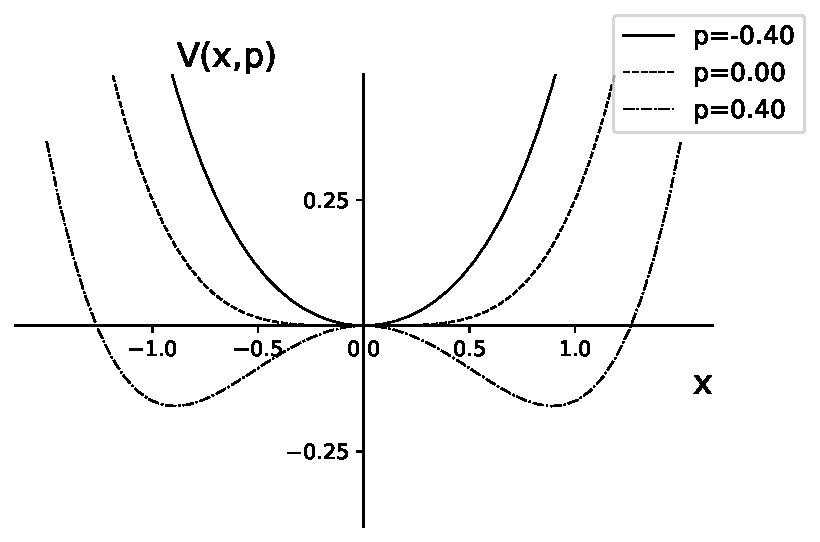
\includegraphics[scale=0.4]{superpitch_p}
		\renewcommand{\figurename}{Fig.}
	\end{minipage} 
	\caption{\small \textbf{Left:} bifurcation diagram of the supercritical pitchfork normal form \ref{eq:suppitch}. The equilibrium manifold is in black (solid line: stable; dashed: unstable).Vector field lines indicate whether the system is pushed upwards or downwards. \textbf{Right:} evolution of $V(x,p)$ for a subcritical pitchfork normal form when $p$ changes from negative to positive values. Notice that the final steady state is with two minima, but the mechanism to reach this state is different from that of a subcritical pitchfork shown in Fig.~\ref{fig:subpitch_global}, centre.}
	\label{fig:superpitch_diagram_bif}
\end{figure}





\tocless\subsection{Cusp}
\label{subsec:cusp}
The cusp is a dimension-1, codimension-2 bifurcation, for which is generic. According to R. Thom's classification of catastrophes \cite{Thom2554}, the cusp is the main ``organising centre'' in one dimension. It is defined according to the conditions:

\begin{align}
	\nonumber & \frac{\partial f}{\partial x}(0,p_0)= \frac{\partial^2 f}{\partial x^2}(0,p_0) = \frac{\partial f}{\partial p}(0,p_0) = \frac{\partial^2 f}{\partial p \partial x}(0,p_0) = 0 \\
	\nonumber & \frac{\partial^3 f}{\partial x^3}(0,p_0) \neq 0\\
\end{align} 

The cusp normal form is:
\begin{equation}
	\dot{x} = a + b x - x^3 \, .
	\label{eq:cusp}
\end{equation}

It can be regarded as an ``intersection'' of supercritical pitchfork and fold bifurcations (see Fig. \ref{fig:cusp}, left), or as an unfolding (Def.~\ref{def:unfolding}) around a supercritical pitchfork bifurcation. The projection of its stable region in the $(a,b)$ plane is shown in Fig. \ref{fig:cusp}, right. Appendix~\ref{app:catasrophe} reports a historical example of a simple toy model displaying cusp-like behaviour, that can be (and was, during the thesis) studied experimentally. 

In this case, CSD is dictated by the direction of evolution, whether it is along the fold or pitchfork eigenvector. \\

\begin{figure}[h!]
	\centering
	\begin{minipage}[c]{0.49\textwidth}
		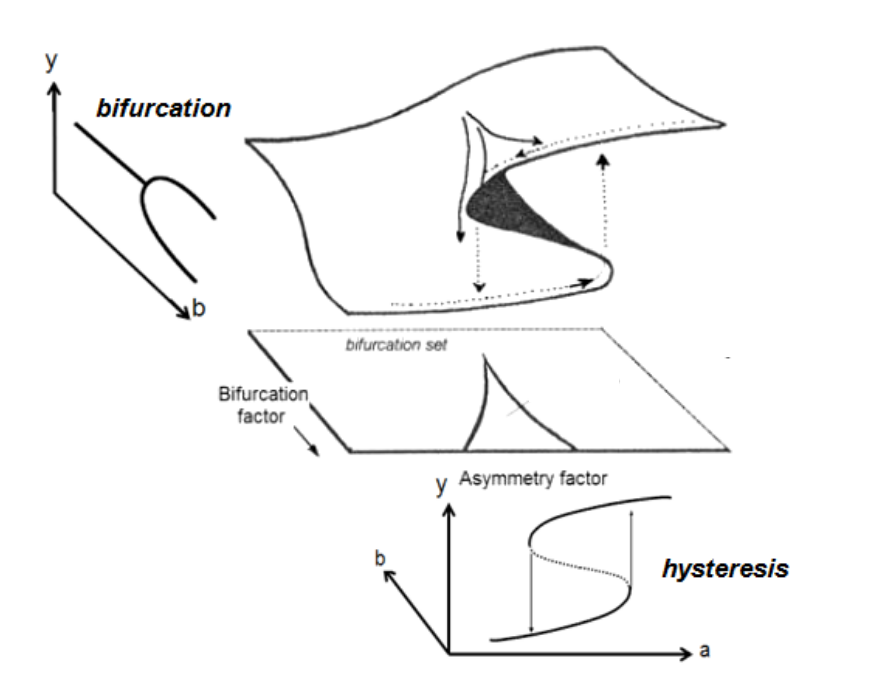
\includegraphics[scale=0.4]{cusp_surface}
		\renewcommand{\figurename}{Fig.}
	\end{minipage}
	\hspace{0.05cm}
	\begin{minipage}[c]{0.49\textwidth}
		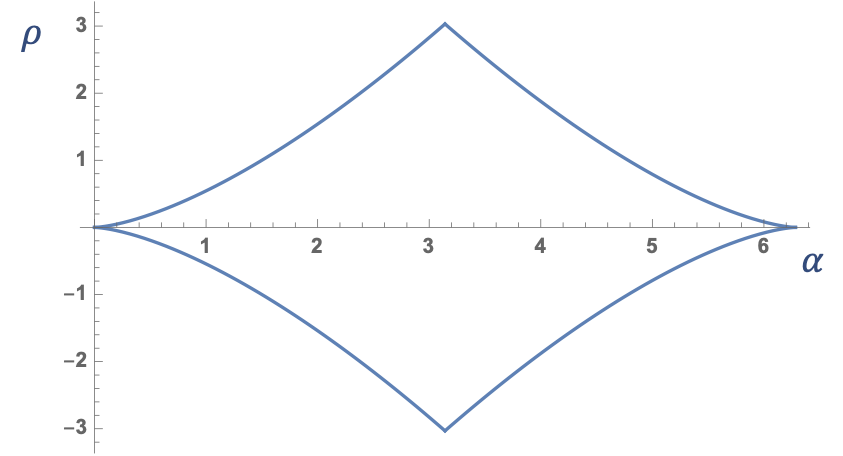
\includegraphics[scale=0.45]{cusp}
		\renewcommand{\figurename}{Fig.}
	\end{minipage} 
	\caption{\small \textbf{Left:} artistic representation of a cusp stable manifold, its projection on the $(a,b)$ plane and the ``intersection'' of supercritical pitchfork and fold bifurcations, according to the direction marked by one or the other parameter. Figure from \textcite{stamovlasis2014bifurcation}. \textbf{Right:} projection of its stable region in the $(a,b)$ plane. Values from Catastrophe Machine (\textit{cf.} Appendix~\ref{app:catasrophe}).}
	\label{fig:cusp}
\end{figure}





\tocless\subsection{Subcritical Hopf}
It is a critical 2-dimensions, 1-codimension bifurcation from stable point to cycle. Its normal form is:
\begin{align}
	\nonumber \dot{x}_1 &= p x_1 - x_2 + l x_1(x_1^2 + x_2^2)\\
	\dot{x}_2 &= x_1 + p x_2 + l x_2(x_1^2 + x_2^2) \, .
	\label{eq:subhopf}
\end{align}
The meta-parameter $l$ is called \textit{Lyapunov coefficient}. Its sign identifies the Hopf criticity ($l>0$ for subcritical, $l<0$ for supercritical).

Its qualitative properties can be obtained by inquiring the subcritical pitchfork, as there exist a change of coordinates that connects the two.
\begin{proof}
	Equations \ref{eq:subhopf} are symmetrical with the $(x_1^2 + x_2^2)$ term that closely resembles a radius. Thus it is natural to ask for a change of coordinates from planar to polar:
	\begin{equation}
		(x_1,x_2) \rightarrow (\rho, \vartheta) \, .
	\end{equation}
	So that:
	\begin{equation}
		\left\{
		\begin{array}{ll}
			x_1 = \rho \cos \vartheta\\
			x_2 = \rho \sin \vartheta
		\end{array}
		\right.
		\label{eq:coordinates}
	\end{equation}
	whose differential is:
	\begin{equation}
		\left\{
		\begin{array}{ll}
			\dot{x}_1 = \dot{\rho} \cos \vartheta - \rho \sin\vartheta \dot{\vartheta}\\
			\dot{x}_2 = \dot{\rho} \sin \vartheta + \rho \cos\vartheta \dot{\vartheta} \, .
		\end{array}
		\right.
		\label{eq:coordinates_diff}
	\end{equation}
	Substituting Eq. \ref{eq:coordinates} and \ref{eq:coordinates_diff} into Eq. \ref{eq:subhopf} gives:
	\begin{equation}
		\left\{
		\begin{array}{ll}
			\dot{\rho} \cos \vartheta - \dot{\vartheta} \rho \sin\vartheta = \cos\vartheta(p\rho + \rho^3) - \rho \sin\vartheta \\
			\dot{\rho} \sin \vartheta - \dot{\vartheta} \rho \cos\vartheta = \sin\vartheta(p\rho + \rho^3) - \rho \cos\vartheta \, . 
		\end{array}
		\right.
	\end{equation}
	Which is valid if:
	\begin{equation}
		\left\{
		\begin{array}{ll}
			\dot{\rho} = p \rho + \rho^3 \\
			\dot{\vartheta} = 1 \, .
		\end{array}
		\right.
	\end{equation}
	That is, if the evolution of the system along the radial parameter follows a subcritical pitchfork bifurcation and the angular speed is constant.
\end{proof}

\textsc{CSD Scaling}
Using the previous result, CSD comes from the very same calculation as that of the pithcfork:
\begin{equation}
	[u' = \partial_\rho(p\rho+\rho^3)|_{\hat{\rho} = 0}u = \mathcal{O}(p) u \ , \ \alpha =1 \, .
\end{equation}




\tocless\subsection{Supercritical Hopf}

It is the ``non-abrupt'' counterpart of the subcritical case. It emerges when complex eigenvalues become zero in their real part. It let a stable point become a fixed cycle in a continuous fashion. Its radial evolution is connected to the supercritical pitchfork by following similar reasoning to that of the subcritical Hopf (see above). Its normal form is:
\begin{align}
	\nonumber \dot{x}_1 &= p x_1 - x_2 + l x_1(x_1^2 + x_2^2)\\
	\dot{x}_2 &= x_1 + p x_2 + l x_2(x_1^2 + x_2^2) \, .
	\label{eq:suphopf}
\end{align}
The meta-parameter $l$ is called \textit{Lyapunov coefficient}. Its sign identifies the Hopf criticity ($l>0$ for subcritical, $l<0$ for supercritical).


\begin{figure}[h]
	\centering
	\begin{minipage}[c]{0.32\textwidth}
		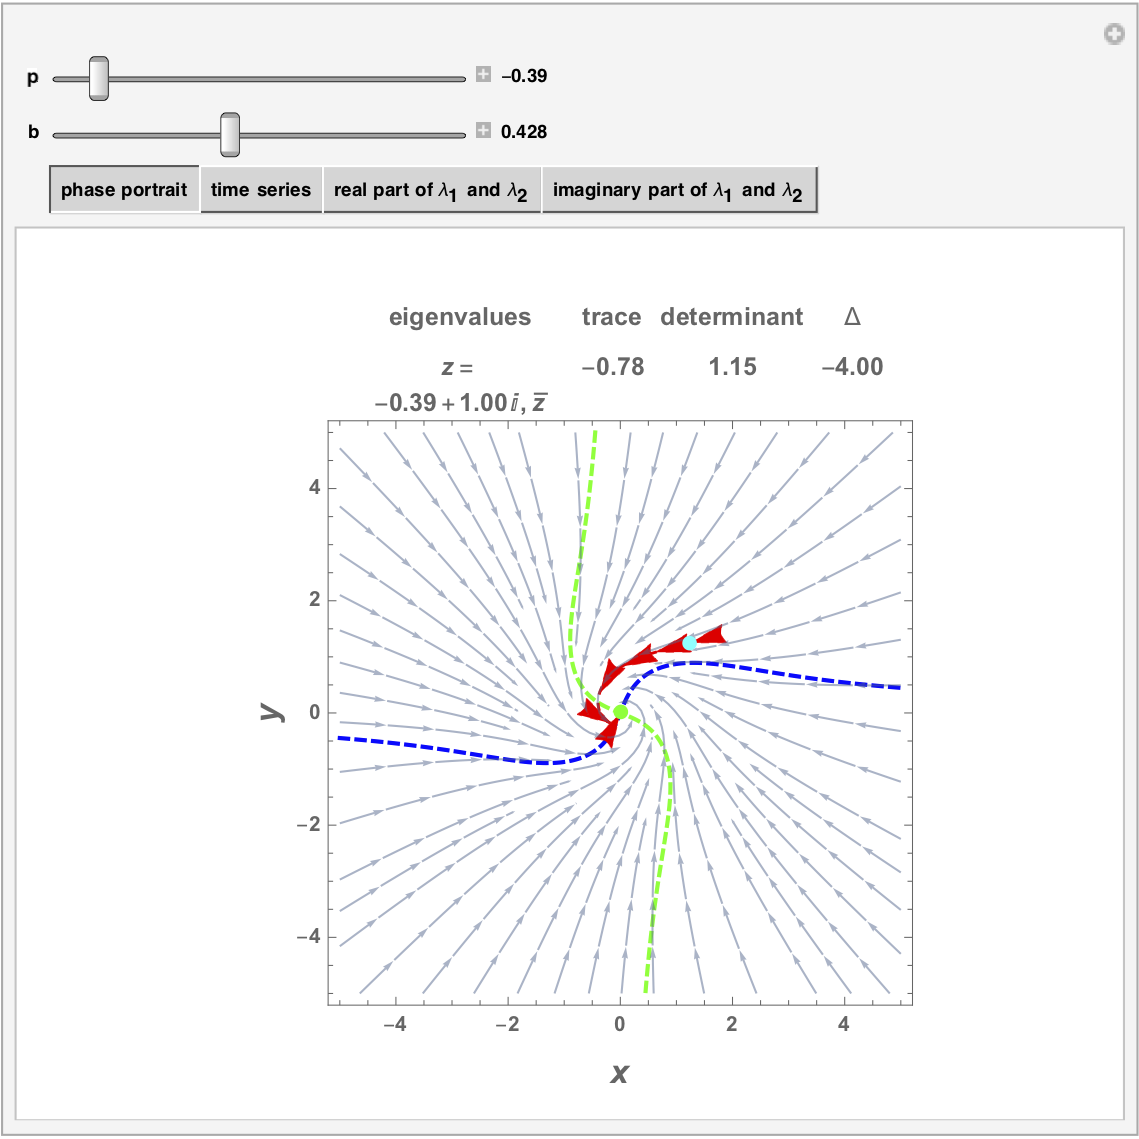
\includegraphics[scale=0.25]{hopf1}
		\renewcommand{\figurename}{Fig.}
		\caption*{$p<0$}
	\end{minipage}
	\hspace{0.05cm}
	\begin{minipage}[c]{0.32\textwidth}
		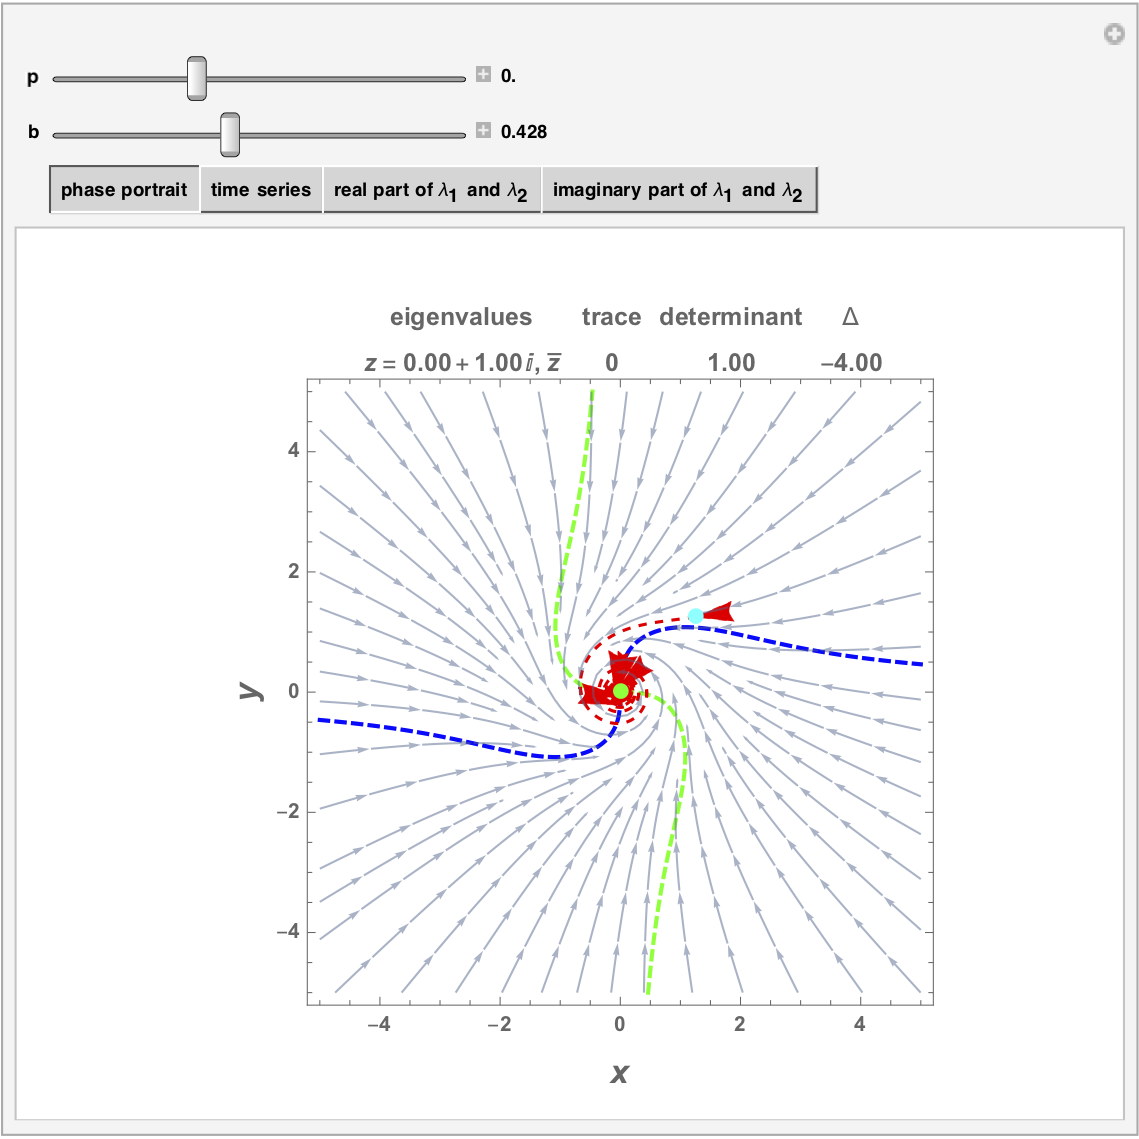
\includegraphics[scale=0.25]{hopf2}
		\renewcommand{\figurename}{Fig.}
		\caption*{$p=0$}
	\end{minipage} 
	\hspace{0.05cm}
	\begin{minipage}[c]{0.32\textwidth}
		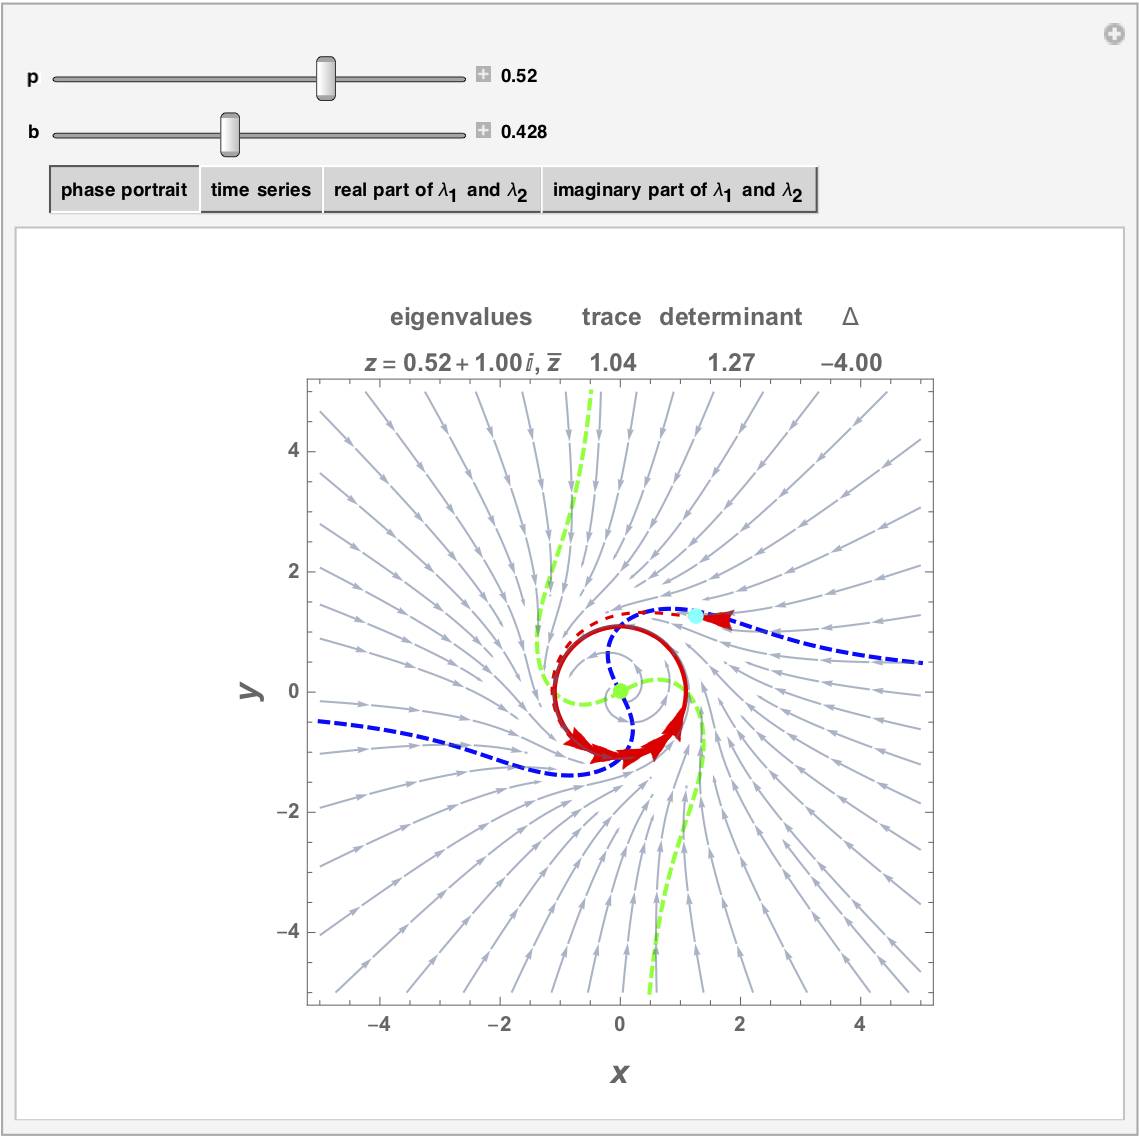
\includegraphics[scale=0.25]{hopf3}
		\renewcommand{\figurename}{Fig.}
		\caption*{$p>0$}
	\end{minipage}
	
	\caption{\small Evolution of the trajectories for a Hopf pitchfork normal form when $p$ changes from negative to positive values, displayed on the phase portrait along $(x_1,x_2) = (x,y)$. $b=-l$ is the (negative) Lyapunov coefficient for subcritical Hopf. For $p<0$, only fixed point solutions are stable. For $p=0$ there is a Hopf point, leading to limit cycles for $p>0$. Discriminant, trace and determinant (\textit{cf.} Sec~\ref{sec:formal_stability}) are also reported. The figures are generated with code adapted from Suba Thomas, "Bifurcation Diagrams with Flow Fields" \url{http://demonstrations.wolfram.com/BifurcationDiagramsWithFlowFields/}, Wolfram Demonstrations Project, Published: March 7 2011.}
	\label{fig:hopf}
\end{figure}

\textsc{CSD Scaling}
Using the previous result, CSD comes from the very same calculation as that of the pithcfork:
\begin{equation}
	[u' = \partial_\rho(p\rho+\rho^3)|_{\hat{\rho} = 0}u = \mathcal{O}(p) u \ , \ \alpha =1 \, .
\end{equation}




\tocless\subsection{Other - possibly critical - bifurcations}
Higher-dimension and -codimension bifurcations exist and can be critical depending on their parameter settings. However, they have not been further considered in this thesis. For completeness, the most relevant ones for continuous systems \citep{kuehn2011mathematical} are listed below.
\begin{itemize}
	\item 
	Bautin (generalized Hopf): 2D, 2c-D (plus Lyapunov parameter $l$ that defines its criticity depending on the sign). Similarly to the Hopf bifurcation, it describes shifts from fixed points to limit cycles. Its normal form is:
	\begin{align}
		\nonumber \dot{x}_1 &= p_1 x_1 - x_2 + p_2 x_1(x_1^2 + x_2^2) + l x_1 (x_1^2 + x_2^2)^2\\
		\dot{x}_2 &= x_1 + p_1 x_2 + p_2 x_2(x_1^2 + x_2^2) + l x_2 (x_1^2 + x_2^2)^2 \, .
		\label{eq:bautin}
	\end{align}
	\item 
	Bogdanov-Takens: 2D, 2c-D (plus Lyapunov parameter $s$ that defines its criticity depending on the sign). It emerges from the coalescence of a saddle-node and a Hopf. Its normal form is:
	\begin{align}
		\nonumber \dot{x}_1 &= x_2\\
		\dot{x}_2 &= p_1 + p_2 x_2 + x_1^2 + s x_1 x_2 \, .
		\label{eq:bog_tak}
	\end{align}
	\item 
	Hopf-fold and Hopf-Hopf (3D, 2 c-D) may be critical depending on parameter settings.
\end{itemize}








\tocless\section{Stochastic Processes}
\label{sec:stochastic_p_formal}

The way scientists model random phenomena (or phenomena that involve random or supposedly randomic processes) is through the theory of stochastic processes. It is a discipline that combines kinetics, dynamical systems, probability theory and information theory to study noise. This section lists a few important concepts that will be used in the thesis. Most of the definitions, as well as more extensive presentations of the discipline and related problems can be found in \citep{freidlin1998random,,Gardiner1985}. This section assumes that the reader is familiar with basic concepts of probability and statistics (suggested further reading in \textcite{papoulis2002probability}). 
\begin{definition}
	A \textbf{random} or \textbf{stochastic} variable $\check{x}$ is a number associated to the outcome of a random phenomenon $\xi$.
	\begin{equation}
		\xi \xrightarrow[]{\check{x}} \check{x}(\xi)
	\end{equation}
\end{definition}
\begin{definition}
	Given a fixed value $x$ and having defined the concept of ``probability''\footnote{Defining probability and discussing its theorems is beyond the scope of this appendix. Refer to \cite{papoulis2002probability} for advanced explanation.}, we define the \textbf{distribution function} $F_x(x)$ as 
	\begin{equation}
		F_x(x) = \mathcal{P}\{\check{x} \leq x\} 
	\end{equation}
Notable property: $F_x(x) \geq 0$ and is monotonously increasing.
\end{definition}
It records all the probabilities implying that a random variable assumes values that are lower than a certain number. Another (more common) way to represent the same concept is by means of the probability density function.
\begin{definition}
	The \textbf{probability density function} is defined as 
	\begin{equation}
		f_x(x) = \frac{dF_x(x)}{dx}
	\end{equation}
Notable property: $f_x(x) \geq 0$. Moreover, $f(x) = \sum_{i} P_i \delta(x-x_i)$ for discrete cases.
\end{definition}

\begin{definition}
	A \textbf{stochastic process} is a rule to associate values to the outcome of a random phenomenon that evolves in time:
	\begin{equation}
		\text{sp}: \xi(t) \rightarrow \check{x}(\xi, t)
	\end{equation}
\end{definition}
There are discrete or continuos stochastic processes, depending on the domain of $t$ and of possible values of $\check{x}$, with different properties. As this thesis focuses on the assumption of variable continuum, only continuous stochastic processes will be considered below. In order to study the evolution of such processes, the most used equations are the associated Langevin equations and their corresponding Fokker-Planck equations, described below. Connecting Langevin equations to fine-grained descriptions like Master equations can be done, e.g. according to Gillespie's formalism \citep{Gillespie2000}, but will not be discussed further.

\begin{definition}
	A \textbf{Wiener process} is a Gaussian process, continuos in time. It models a Brownian motion (random motion with independent increases). It is identified as the integral of a white noise process (stochastic process with zero mean).
\end{definition}

\begin{definition}
	An equation that takes into account the deterministic driving force of a process and its stochastic component (often in the form of white noise) is called the associated \textbf{Langevin equation} to that process. Its general form is:
	\begin{equation}
		\dot{x_i} = \frac{dx_i}{dx} = a_i(\bar{x}) + \sum_{m=1}^{n}b^m_i(\bar{x})g_m(t)
	\end{equation}
	where the superscript $\check{}$ was dropped for simplicity. $a_i$ and $b_i$ are generic functions. $g_m(t)$ are random functions, typically the derivative of a Wiener process $dW$. In terms of differential forms, a Langevin equation reads:
	\begin{equation}
		du  = a(x) \, dt + b(x) \, dW
		\label{eq:langevin_eq}
	\end{equation}
\end{definition}

The general form of a Langevin equation can be more complicated and can involve differently ``coloured'' noise, or noise that is state-dependent or has other properties. It can be solved with different techniques and its moments can also be estimated if the distribution of every $g_m(t)$ is known.\\
The Langevin equation describes the evolution of the process. The evolution of its associated probability density function (meaning the rule to transit from one state to another), on the other hand, is given by the associated Fokker-Planck equation.

\begin{definition}
	The associated \textbf{Fokker-Planck equation} to a stochastic process is a diffusion equation for its probability density function  $P$ that locally approximates an It\^{o} stochastic differential equation. In its simplest form it reads:
	\begin{equation}
		\partial_t P(x,t | x_0, t_0) = - \partial_x \left[A(x,t) P(x,t | x_0, t_0) \right] + \frac{1}{2} \partial^2_x \left[B(x,t)^2 P(x,t | x_0, t_0) \right]
		\label{eq:fokker_plank}
	\end{equation}
	where $P(x,t | x_0, t_0)$ is the ``probability to go to value $x$ at time $t$ given the value $x_0$ at time $t_0$, $A(x,t)$ is a ``drift'' term that accounts for the deterministic forces acting on the system and $B(x,t)$ is a diffusion term.
\end{definition}
Obviously, Eq. \ref{eq:fokker_plank} can be extended to its multivariate case. As a PDE, it can be rarely solved analytically (most of the time by means of path integral techniques) unless one considers its stationary values ($\partial_t P =0$). Boundary conditions need to be specified. In case of multiplicative noise ($b(u) \neq \text{const}$ in Eq. \ref{eq:langevin_eq}), $A$ and $B$ can be combinations of $a$ and $b$ \citep{Risken1991}. 

\begin{definition}
	Let us consider stationary processes in which $a(x) = -\frac{\partial V(x)}{\partial x}$ (case of a potential well) and $b(x,t) = \sqrt{2D}$. An \textbf{Ornstein-Uhlenbeck process} is then defined as 
	\begin{equation}
		du = -k \, u \, dt + \sqrt{2D} \, dW
		\label{eq:o-u}
	\end{equation}
	or, alternatively, by its Fokker-Planck representation
	\begin{equation}
		\partial_t P = \partial_x (kxP) + D \, \partial^2_x P \, .
	\end{equation}
\end{definition}


Linking stochastic processes (driven by pure noise) to slow-fast systems (\ref{eq:slowfast}) is not trivial. Khasminskii was among the first to suggest that the effect of fast degrees of freedom on the slow variable dynamics could be approximated as noise term \citep{khas1966limit}. Later on, various scholars \citep{namachchivaya1990equivalence} assessed the equivalence of stochastic averaging and stochastic normal forms. Nowadays, it is a widely employed first approximation \citep{Berglund2006} to model fast fluctuations as stochastic processes on top of the slowly varying degrees of freedom. The ``double nature'' encompassed by such modelling (genuine random realizations and fast dynamics) can be tackled by specifying functional forms for the noise terms, which might be described by non-Gaussian distributions or non-Markovian processes.





\tocless\section{Graphs and Networks}
\label{sec:graphs}
Definitions are adapted from \textcite{gross2005graph,boccaletti2006complex}.

\begin{definition}
	A \textbf{graph} is a triple $(V,E,I)$, where $V$ and $E$ are finite sets, called the vertices and the edges, respectively, and $I:E\to V^2×{0,1}$ is called the incidence function. The incidence function tells for each edge its end-vertices, and whether the edge is directed (1) or not (0). 
\end{definition}
If an edge $e$ is directed, then the first element and the second element of $I(e)$ denote the origin vertex and the destination vertex, respectively. This generality is required to represent all of undirected graphs, directed graphs, and mixed graphs, possibly combined with self-loops and multi-edges.

\begin{definition}
	A \textbf{labeled graph} is a graph together with labeling functions $L_V:V \rightarrow D_V$ and $L_E:E \rightarrow D_E$, where $D_V$ and $D_E$ are arbitrary sets, called the vertex labels and the edge labels, respectively
\end{definition}

\begin{definition}
	A \textbf{network} is the realistic counterpart of a mathematical graph. It may have an associated dynamics, links can have associated functions for activation and so on. 
\end{definition}
As long as we bear in mind that ``graph'' is a topological representation whereas ``network'' is also involving dynamics, they can be used pretty much interchangeably. Just recall the following terms \citep{barabasi2016network}:

\begin{table}[h!]
	\centering
	\begin{tabular}{c|c }
		\textbf{Network Science} & \textbf{Graph Theory}   \\ \cline{1-2}
		Network                  & Graph                  \\ 
		Node                     & Vertex                  \\
		Link                     & Edge                    \\
	\end{tabular}
\end{table}



\tocless\section{Microstate and macrostate}
\label{sec:micro_macrostate}
``Macrostate'' and ``microstate'' are terms derived from Statistical Mechanics. An intuitive outline that extends the more formal definition from physics \citep{pathria} is:


\begin{definition}
	A \textit{microstate} is a specific configuration of individual constituents that, once coupled, give rise to emerging macrostates.
\end{definition}
In thermodynamics, given a system with $\mathcal{D}$ degrees of freedom and its phase space $\Omega=(q_i,p_i)$, the microstate is specified by a single point in the phase space. $q_i$ are generalised coordinates and $p_i$ the generalised momenta. When $\mathcal{D} \to \infty$, the phase space can be divided into cells of size $\Delta_0 = \Delta q_i \Delta p_i$, each treated as a microstate. Similar reasoning can be put forward for other systems, where the generalised coordinates relate to other quantities. For instance, gene regulatory networks can be described in gene state spaces \citep{wu2020nowcasting}, where each combination of gene expression levels can be treated as a microstate.

\begin{definition}
	A \textit{macrostate} of a system refers to its macroscopic (possibly emergent) properties that account for its function, such as temperature or density. 
\end{definition}


Overall, a macrostate is what results from interactions of single components of a complex system. It is an ``emerging'' property. In statistical mechanics, different configurations of molecule speeds (its microstate) create a single temperature value (associated macrostate). Any given macrostate may be associated with many different microstates.
		
Example: for a biological system, we can think of a macrostate as a functional state. Importantly, it can be observed and measured. We conjecture that gene expression profiles can be related to microstates in a biological context. These are often inferred. If a circuit is known, we can think of its control parameters as microstates, as different combinations may produce the same outcome (e.g. the same function, or macrostate).


